\documentclass[a4paper,12pt]{article}

\title{Biology 30 IB \\ Cells, Chromosomes, \& DNA}
\author{Jad Chehimi}

% document setup
\renewcommand{\familydefault}{\sfdefault}
\linespread{1.25}
\usepackage[margin=1in]{geometry}
\usepackage{setspace}
\usepackage{enumitem}
\setlist{nosep}
\usepackage{amsmath}
\usepackage{color,soul}
\setcounter{secnumdepth}{0}
\usepackage{wasysym}

% tools
\usepackage[hidelinks]{hyperref}
\usepackage{float}
%% images
\usepackage{graphicx}
\graphicspath{ {./images/} }
%% science
\usepackage{siunitx}

\begin{document}
\maketitle

\section{Resources}
\begin{itemize}
    \item{\href{https://docs.google.com/document/d/1-Agcr85pflQCNP3PUO7vbdybJLy7BT0y3zjFPgRvhuI}{Videos and Animations}}
\end{itemize}

\tableofcontents

\pagebreak

\section{Terms}
\begin{itemize}
    \item{\textbf{Somatic cells} are all cells in the body \hl{except sex cells} --- sperm and egg cells}
    \item{A human somatic cell has \hl{46 chromosomes}}
    \item{\textbf{Cell division} is done by Eukaryotic cells --- have a nucleus}
    \item{\textbf{Binary fission} is done by Prokaryotic cells --- have no nucleus, such as \hl{bacteria}}
\end{itemize}

\section{(17.1) Cell Division}
\subsection{Purpose}
\begin{itemize}
    \item{Unicellular organisms (i.e. \hl{zygote}) $\longrightarrow$ Multicellular organisms}
    \item{Growth and maintenance of body cells --- \hl{replacement} of worn out cells}
\end{itemize}

\subsection{Chromosomes}
\begin{itemize}
    \item{
            Comprised of...
            \begin{itemize}
                \item{nucleic acids (DNA)}
                \item{proteins}
            \end{itemize}
        }
    \item{
            Either...
            \begin{itemize}
                \item{\textbf{Uncondensed} aka. \textbf{Chromatin} = long, thin strands. invisible to microscope}
                \item{\textbf{Condensed} = thick \& shortened. visible to microscope}
            \end{itemize}
        }
\end{itemize}

\subsection{Chromatid}
\begin{itemize}
    \item{The strand that makes up a normal chromosome}
    \item{
            In mitosis...
            \begin{itemize}
                \item{A chromosome duplicates into two \hl{identical} chromatids, joined together by a \textbf{centromere}, to form a \textbf{duplicated chromosome}}
                \item{These chromatids are referred as \textbf{sister chromatids} in this state}
                \item{Each chromatid of a duplicated chromosome goes to each of the two new cells}
            \end{itemize}
        }
\end{itemize}

\begin{figure}[H] 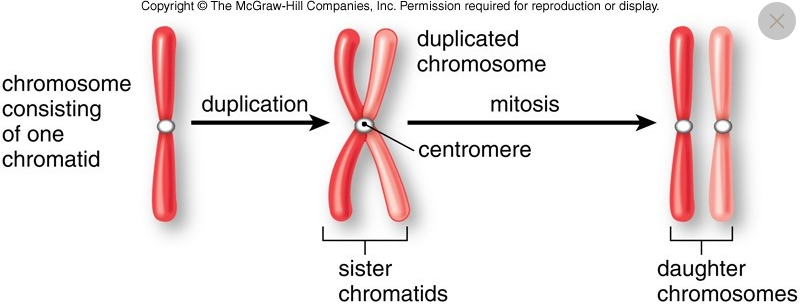
\includegraphics[width=0.9\textwidth]{chromosome} \end{figure}

\section{Cell Cycle}
\begin{figure}[H] 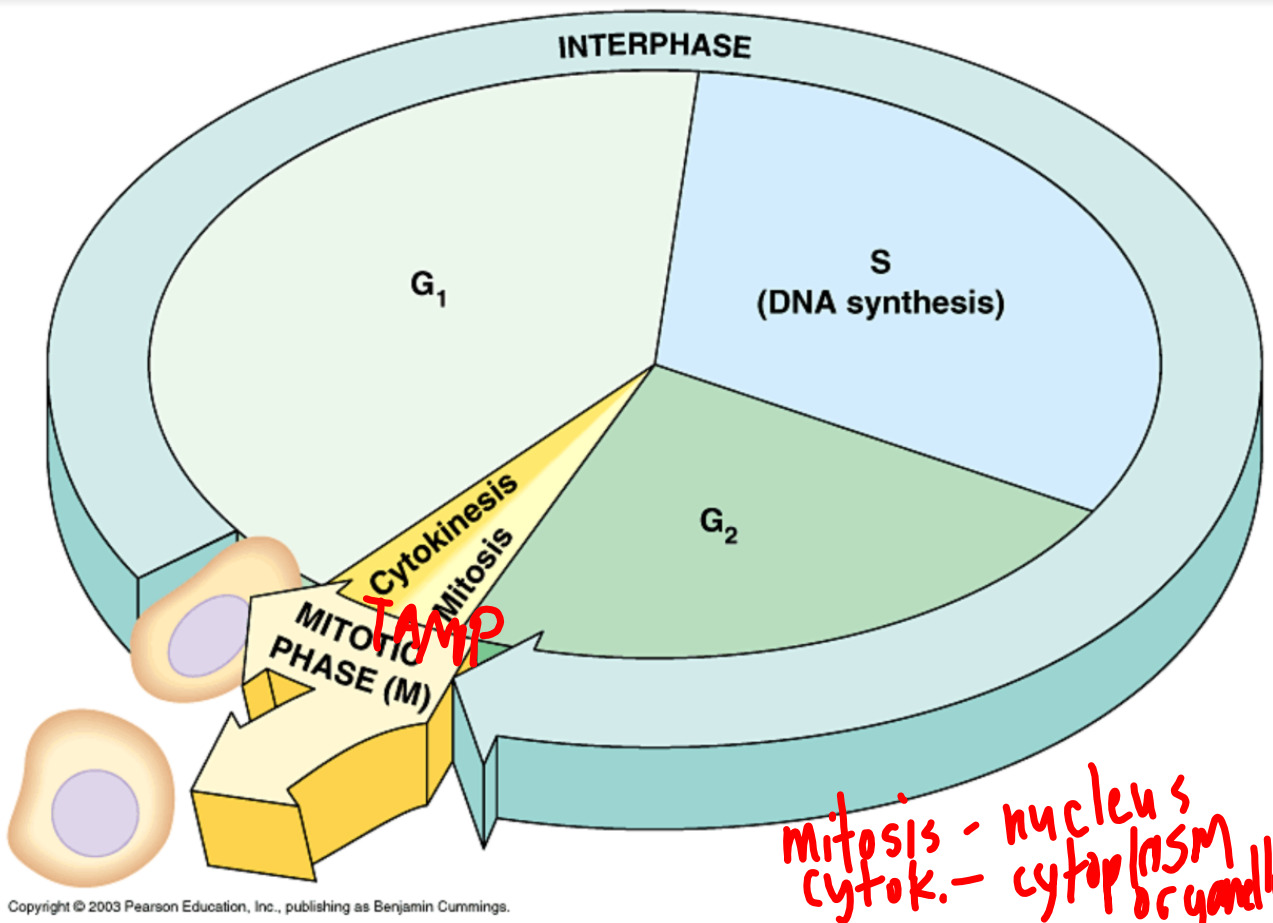
\includegraphics[width=0.9\textwidth]{cellcycle} \end{figure}

A continuous cycle that involves all steps of a cell's life, especially cell division.

\subsection{Interphase}

\hl{MAJOR PHASE}

\begin{itemize}
    \item{90\% of cell cycle}
    \item{All cell activity when not dividing}
\end{itemize}

\subsubsection{Gap 1 ($G_1$)}
\begin{itemize}
    \item{Cell growth and general function}
    \item{After cell division, cells may be smaller than their parent. Cell growth is needed}
\end{itemize}

\subsubsection{S Phase ($S$)}
\begin{itemize}
    \item{DNA is doubled}
    \item{Single(-chromatid) chromosome $\xrightarrow{\textrm{duplication}}$ double(-chromatid) chromosome}
\end{itemize}

\subsubsection{Gap 2 ($G_2$)}
\begin{itemize}
    \item{Organelles are doubled, and proteins for the new cell are produced}
\end{itemize}

\subsection{Mitotic Phase}\noindent

\hl{MAJOR PHASE}; occurs in somatic cells.

Distribution of \hl{nucleus and its contents}.

\subsubsection{Prophase}
\begin{itemize}
    \item{Chromatin condense --- shorten \& thicken --- into chromosomes, becoming visible}
    \item{Nuclear membrane fades}
    \item{
            Animal cells only...
            \begin{itemize}
                \item{\textbf{Centrioles} (aka. centrosomes) move to opposite poles of cell. (N/S, E/W)}
                \item{Two centrioles are at each pole, total four, for each cell}
                \item{Centrioles deploy \textbf{spindle fibers}}
            \end{itemize}
        }
    \item{Without centrioles --- such as plant cells --- spindle fibers are still present and the cycle works the same}
\end{itemize}

\begin{figure}[H]
    \centering
    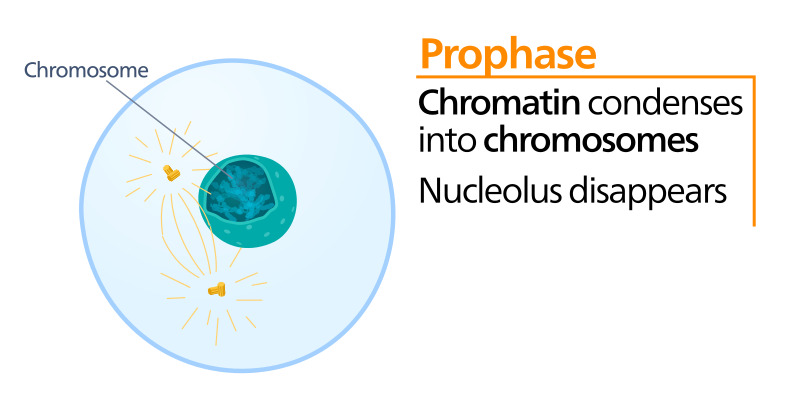
\includegraphics[width=0.5\textwidth]{prophase}
\end{figure}

\subsubsection{Metaphase}
\begin{itemize}
    \item{\textbf{Equatorial plate} = center of cell}
    \item{Sister chromatids move towards equatorial plate}
    \item{Chromosomes attach to spindle fibers}
\end{itemize}

\begin{figure}[H]
    \centering
    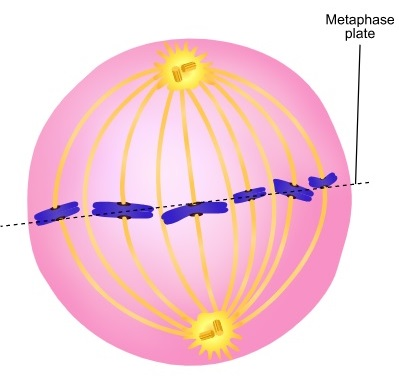
\includegraphics[width=0.5\textwidth]{metaphase}
\end{figure}

\pagebreak

\subsubsection{Anaphase}
\begin{itemize}
    \item{Centromeres divide}
    \item{(Now) chromatids move towards spindle fibers --- i.e. opposite poles of cell}
\end{itemize}

\begin{figure}[H]
    \centering
    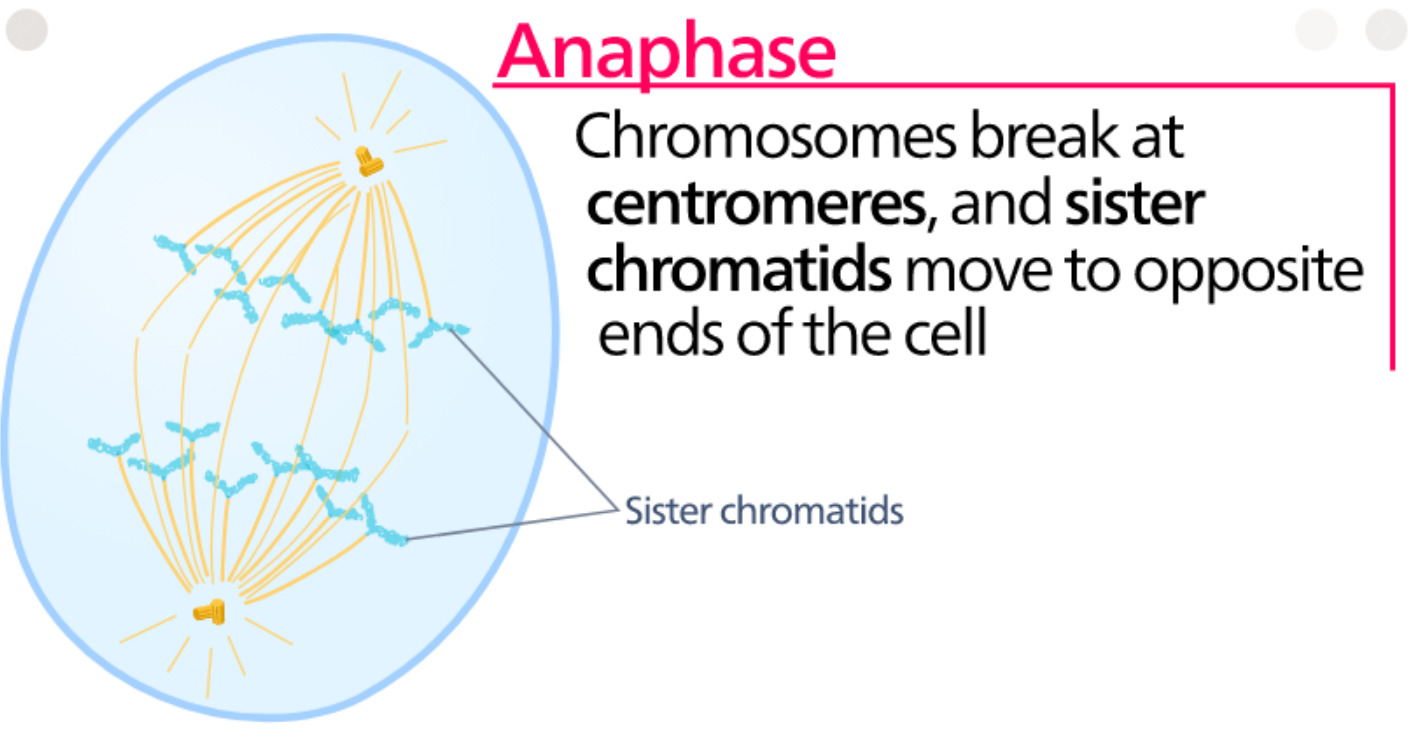
\includegraphics[width=0.75\textwidth]{anaphase}
\end{figure}

\subsubsection{Telophase}
\begin{itemize}
    \item{Spindle fibers dissolve}
    \item{Nuclear membrane forms around each mass of chromatin}
\end{itemize}

\subsubsection{Cytokinesis}
Technically occurs at the end of telophase.
\begin{itemize}
    \item{\hl{Division of cytoplasm} and \hl{distribution of organelles} to "daughter" cells}
    \item{Involves \textbf{cleavage}, pinching off in the center as the cytoplasm moves to opposite poles}
    \item{In plant cells only, a \textbf{cell plate} is distributed, which develops into a new cell wall}
\end{itemize}

\begin{figure}[H]
    \centering
    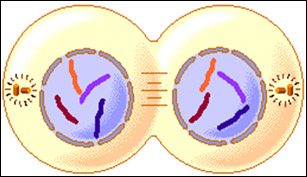
\includegraphics[width=0.75\textwidth]{telophase}
\end{figure}

\section{Cell Properties}

\subsection{Biological Clock}\noindent

Immature cells always have \hl{50 division}, regardless of...
\begin{itemize}
    \item{duration frozen}
    \item{stage/phase that cell division was suspended}
\end{itemize}

\subsection{Death \& Aging}\noindent

Cells may stop dividing due to...
\begin{itemize}
    \item{\textbf{Senescence} = aging, irreversible changes that eventually lead to death}
    \item{\textbf{Specialization} = the more \hl{specialized/differentiated} a cell is, the less likely it will undergo mitosis}
\end{itemize}

Cells that avoid aging are...
\begin{itemize}
    \item{\textbf{Spermatogonia} = sperm-producing cells, immature \& unspecialized}
    \item{Cancer cells of a tumor, which do not become specialized}
\end{itemize}

\pagebreak

\section{(17.2) Natural Cloning}
\begin{itemize}
    \item{Asexual/nonsexual reproduction}
    \item{Identical offspring from a single cell}
\end{itemize}

\subsection{Twins}
\begin{figure}[H]
    \centering
    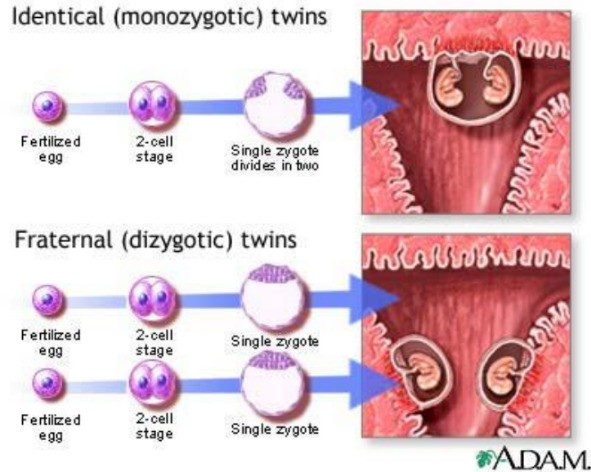
\includegraphics[width=\textwidth]{twins}
\end{figure}

\subsection{Identical Twins}
\begin{itemize}
    \item{Originate from single egg cell}
    \item{During mitosis, \hl{one of the cells breaks free}; this cell forms a 2nd embryo}
    \item{If cell clusters remain separate, two babies with identical gene structures will develop}
    \item{Same gender, blood type, similar facial structure (nature vs. nurture)}
\end{itemize}

\subsection{Fraternal Twins}
\begin{itemize}
    \item{Two different eggs fertilized by different sperm cells}
    \item{Not to be confused with identical twins --- do not have identical genes}
\end{itemize}

\pagebreak

\section{Unnatural Cloning}

A \textbf{totipotent} nucleus is a nucleus that is able to bring a cell from \hl{egg to adult}.

\subsection{Plant Cloning}
\begin{itemize}
    \item{useful, since cloned plants have predictable characteristics}
    \item{requires \hl{delaying cell specialization}}
\end{itemize}

\subsection{Animal Cloning}
\begin{itemize}
    \item{With a micropipette, the nucleus is extracted from an unfertilized egg cell\\The cell is now \textbf{enucleated} (no nucleus)}
    \item{Remove nucleus from a cell of another frog}
    \item{Insert egg cell nucleus into said cell}
    \item{If cell is in \textbf{blastula} stage --- hollow ball of cells of an embryo, early embryo --- then the cells divide into an adult frog, a clone of the frog that donated the \hl{egg cell nucleus}}
    \item{If cell is past blastula --- such as the later \textbf{gastrula} stage --- the cells have \hl{already specialized}, so they do not divide, and the embryo dies}
\end{itemize}

\begin{figure}[H]
    \centering
    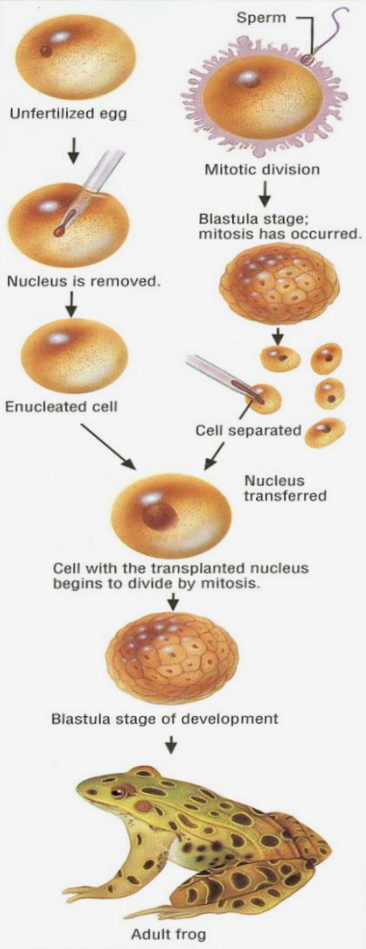
\includegraphics[width=0.3\textwidth]{clone}
\end{figure}

\subsubsection{Mammal Cloning}
\begin{itemize}
    \item{More difficult}
    \item{Cells tend to be \hl{more specialized}}
    \item{Nucleus transfer must be done before 8 cell stage of development}
    \item{Ensures nuclei are totipotent}
    \item{Needs \textbf{surrogate} --- implanting an embryo into a surrogate and having the surrogate birth the offspring. No genetics from surrogate transfer.}
\end{itemize}

\begin{figure}[H]
    \centering
    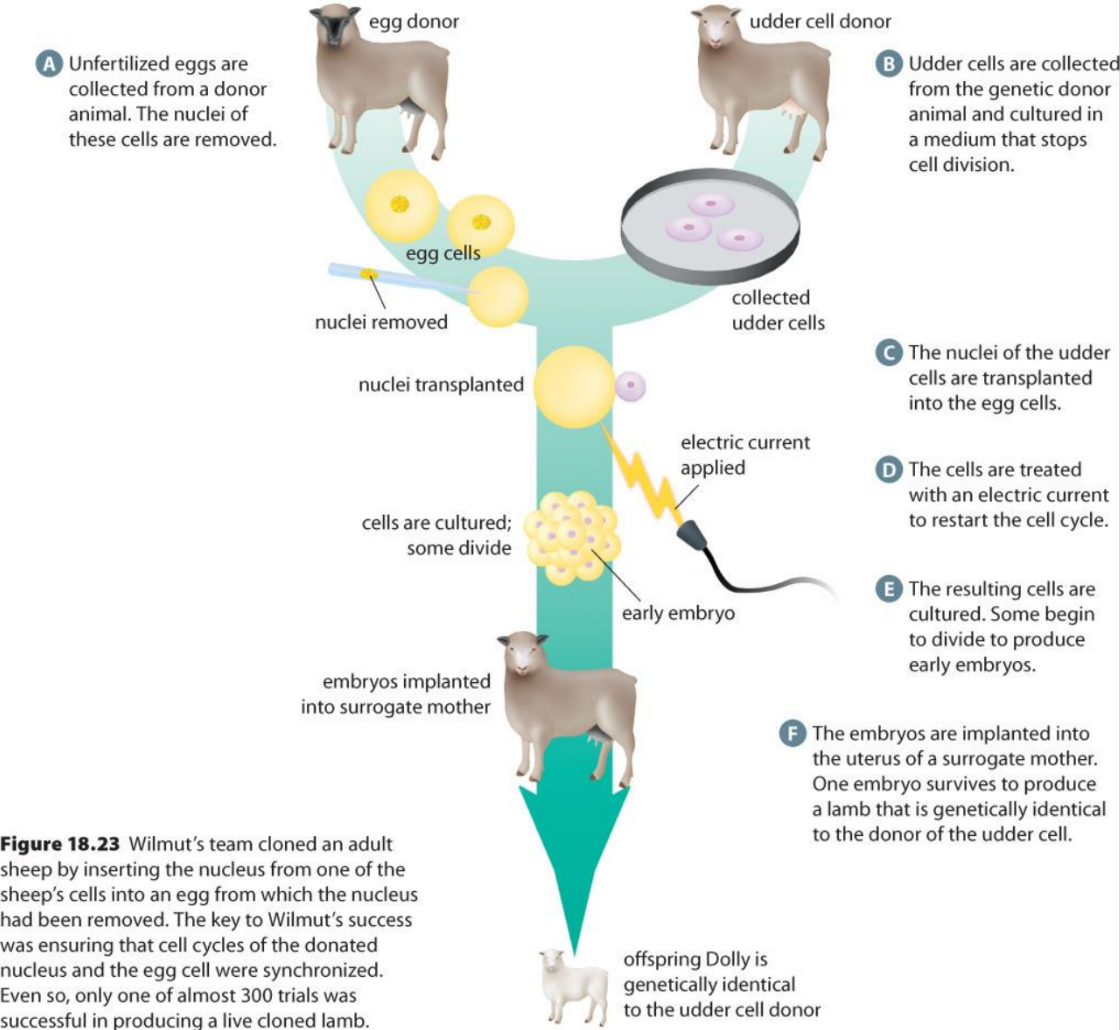
\includegraphics[width=\textwidth]{clone2}
\end{figure}

\pagebreak

\section{Cancer}
\begin{itemize}
    \item{Rapid, uncontrollable growth of cells}
    \item{\hl{Divide faster than normal cells}}
    \item{Some are very slow, some pause and return after many years}
    \item{\hl{Reproduce without directions} from adjacent cells}
    \item{\hl{Cannot specialize} --- making them inefficient}
\end{itemize}

\subsection{Metastasis}
\begin{itemize}
    \item{Cancer cells can dislodge from a tumor and \hl{move to another area}}
    \item{Difficult to isolate source of cancer}
\end{itemize}

\subsection{Tumors}\noindent

A mass of cancerous cells within otherwise normal tissue.

\begin{itemize}
    \item{
            \textbf{Benign Tumor}

            \begin{itemize}
                \item{If cancerous cells remain at site}
                \item{Do not cause serious problems}
                \item{Can be removed by surgery}
            \end{itemize}
        }
    \item{
            \textbf{Malignant Tumor}

            \begin{itemize}
                \item{If cancerous cells metastasize --- dislodge \& travel --- and cause \hl{impairment of other organs}}
                \item{Unusual number of chromosomes}
            \end{itemize}
        }
\end{itemize}

\subsection{Causes}
\begin{itemize}
    \item{x-rays}
    \item{chemical poisons}
    \item{asbestos}
    \item{fungi}
    \item{oncoviruses}
    \item{environmental factors (nature, e.g. diet)}
    \item{age}
    \item{inherited mutations}
\end{itemize}

\subsection{Methods of Identification}
\begin{itemize}
    \item{x-rays}
    \item{cell biopsies}
    \item{infrared technology}
\end{itemize}

\section{Telomeres}
\begin{itemize}
    \item{Caps at the end of chromosomes}
    \item{\hl{Reduce in length every cell cycle/division}}
    \item{Clones --- like Dolly --- inherit their parents telomere length, \hl{shortening their life span} compared to non-clones} 
\end{itemize}

\begin{figure}[H]
    \centering
    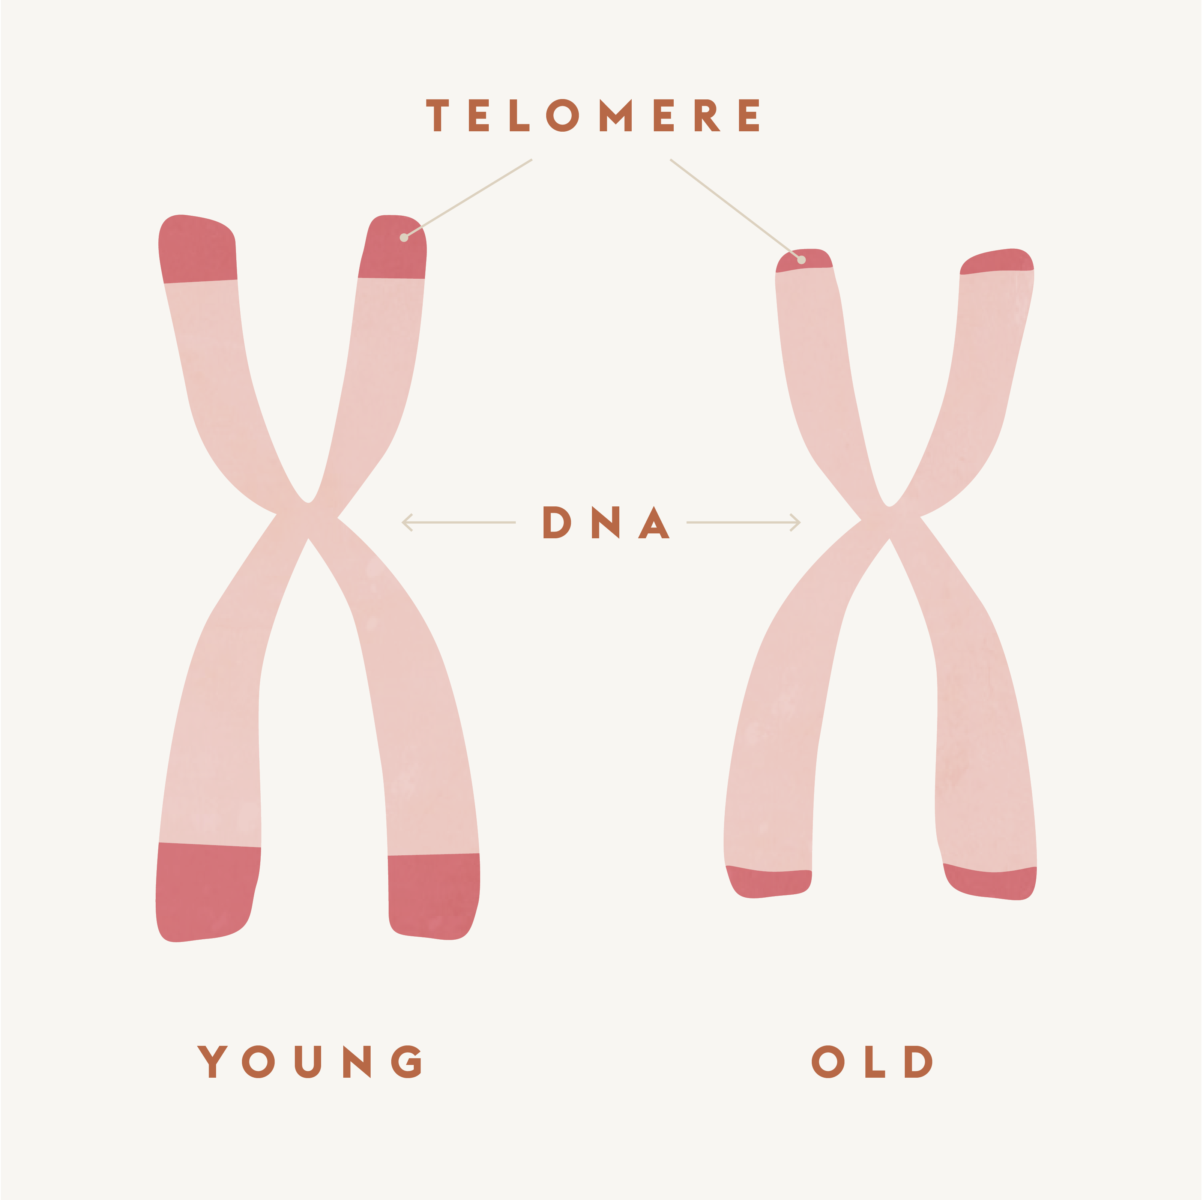
\includegraphics[width=0.50\textwidth]{telomere}
\end{figure}

\subsection{Telomerase}
\begin{itemize}
    \item{An enzyme that \hl{maintains telomere length}, slowing cell death}
    \item{Not present in most normal cells}
    \item{Reactivated in cancer cells, explaining their immortality}
\end{itemize}

\section{(17.3) Sexual Cell Reproduction}

\subsection{Cons}
\begin{itemize}
    \item{consumes a lot of energy}
    \item{infections}
    \item{only half of the genes are passed (not necessarily a con)}
    \item{males are deadbeat --- contribute little to survival of offspring}
\end{itemize}

\subsection{Pros}
\begin{itemize}
    \item{Genetic diversity --- more potential for survival if environmental conditions change.}
    \item{
            Genetic diversity comes from...
            \begin{itemize}
                \item{independent assortment --- random shuffling and random order of genes in meiosis (metaphase I)}
                \item{crossing-over in meiosis (prophase I)}
                \item{random fertilization, combining genes of two separate individuals}
            \end{itemize}
        }
    \item{Two sets of chromosomes, so any damaged DNA has a \hl{backup}, and a \hl{template} to base \hl{DNA repairs} off of}
\end{itemize}

\section{Meiosis}
\begin{itemize}
    \item{\textbf{Gametes} = sex cells --- \female\! ova/ovum (eggs) and \male\! sperm cells}
    \item{\textbf{Gonads} = reproductive organs --- cells of \female\! ovaries and \male\! testes}
    \item{\textbf{Meiosis} = the process of forming gametes}
    \item{\textbf{Autosomes} = chromosomes not directly influenced by sex}
        \\
    \item{\textbf{Diploid} ($2n$) = cell --- such as \hl{somatic cells} --- with a typical \# of chromosomes, such as \hl{46 chromosomes in a human cell}}
    \item{\textbf{Haploid} ($n$) = cell --- such as \hl{gametes} --- with half the typical \# of chromosomes, such as \hl{23 chromosomes in a human gamete}}
\end{itemize}

Meiosis occurs in the germ cells of gonads.

\begin{figure}[H]
    \centering
    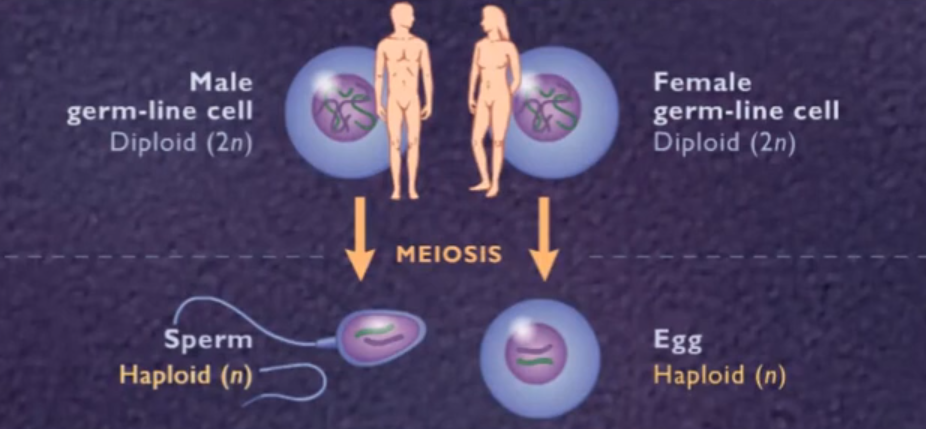
\includegraphics[width=\textwidth]{loid}
\end{figure}

\subsection{Composition of Cells}

\subsubsection{Gametes}
\begin{itemize}
    \item{22 autosomes}
    \item{
            1 sex chromosome
            \begin{itemize}
                \item{Ova can \hl{only} have \female X}
                \item{Sperm can have \hl{either} \female X or \male Y}
            \end{itemize}
        }
    \item{\hl{23 total chromosomes}}
\end{itemize}

\begin{figure}[H]
    \centering
    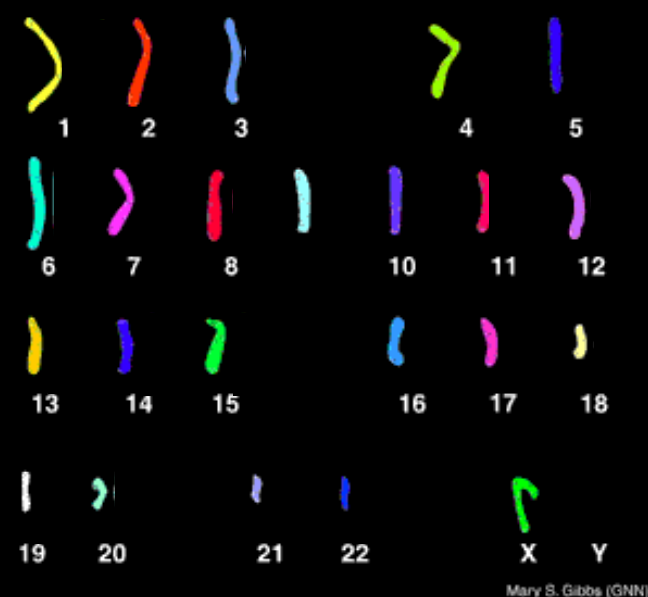
\includegraphics[width=0.45\textwidth]{23}
    \caption{If this were a sperm cell, and it fertilized an egg, the baby would be female}
\end{figure}

\subsubsection{Somatic}
\begin{itemize}
    \item{22 autosome \hl{pairs}}
    \item{2 sex chromosomes --- either \female XX or \male XY}
    \item{\hl{46 total chromosomes}}
\end{itemize}

\begin{figure}[H]
    \centering
    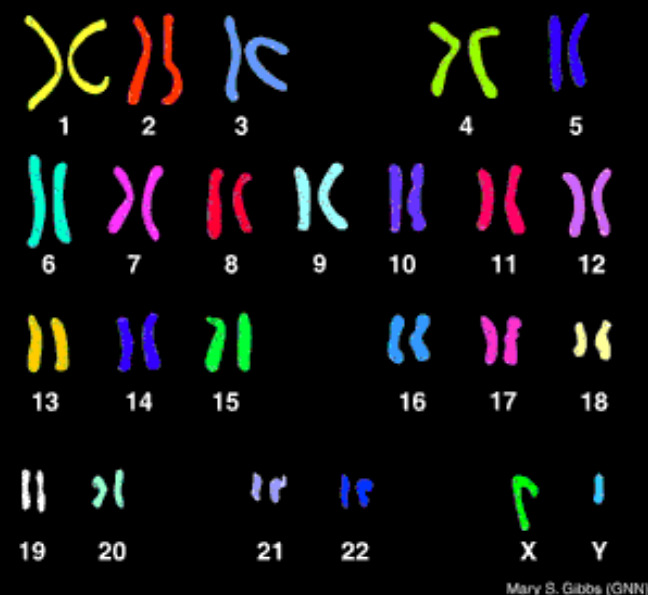
\includegraphics[width=0.45\textwidth]{46}
\end{figure}

\subsection{Union}
\begin{itemize}
    \item{\;\;\;\;23 chromosome (haploid) sperm cell from \male\! male}
    \item{+ 23 chromosome (haploid) egg cell \;\;\,\,\,from \female\! female}
    \item{= 46 chromosome (diploid) zygote or fertilized egg}
\end{itemize}

\section{Stages of Meiosis}

\subsection{Interphase (same as mitosis)}
\begin{itemize}
    \item{Not splitting}
    \item{Important part: S phase --- doubling 46 single chromosomes}
    \item{Ends up as 46 duplicated chromosomes (92 chromotids)}
\end{itemize}

\subsection{Meiosis I}

\subsubsection{Prophase I}
\begin{itemize}
    \item{Same beginning as mitosis
          \begin{itemize}
              \item{Nuclear membrane dissolves}
              \item{Centrioles move to opposite poles of cell, deploying spindle fibers}
          \end{itemize}
         }
     \item{\textbf{Homologous} = \hl{similar} --- such as shape, size, gene arrangement --- but \hl{not identical}}
     \item{Homologous chromosome pairs, one from the mother and one from the father, undergo \textbf{synapsis} --- pairing side by side}
     \item{This forms a \textbf{tetrad} --- 4 chromatids, homologous chromosome pair}
     \item{Chromosomes from the male and female \hl{shuffle around}, as well as \textbf{crossover}}
\end{itemize}
\textbf{Cross-Over}
\begin{itemize}
     \item{Inner chromatids of both chromosomes \textbf{cross-over} --- genetic recombination, exchange genetic information}
     \item{Chromatids of both chromosomes are \hl{no longer sister chromatids} after this point, \hl{not identical}}
\end{itemize}

\begin{figure}[H]
    \centering
    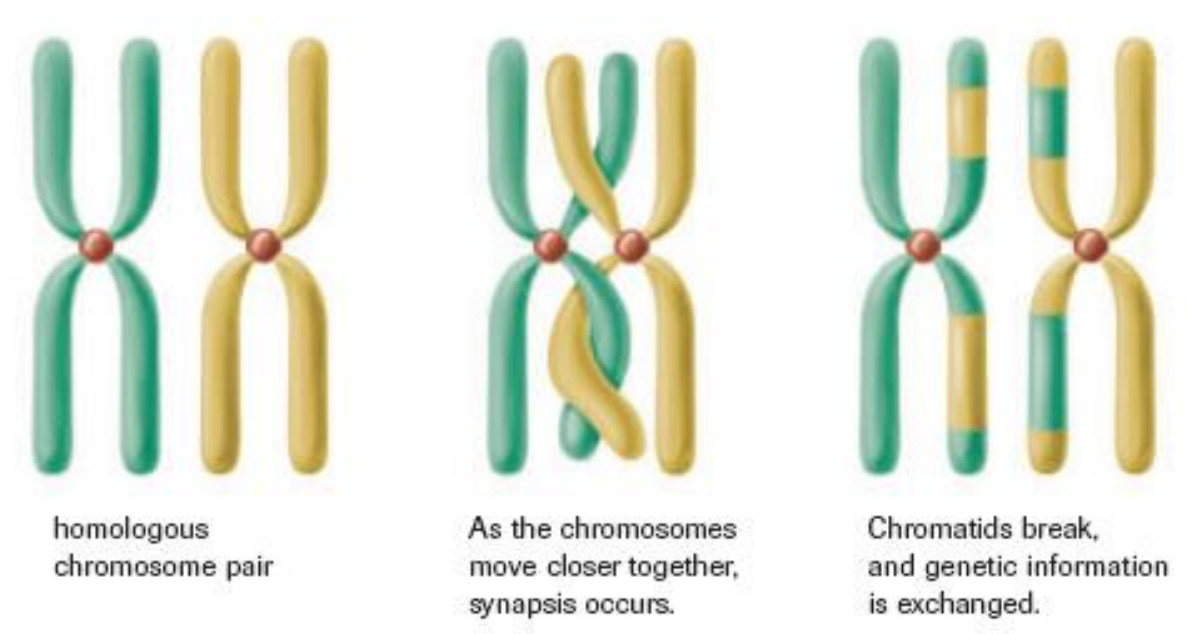
\includegraphics[width=0.6\textwidth]{synapsis}
\end{figure}

\subsubsection{Metaphase I (mostly same as mitosis)}
\begin{itemize}
    \item{Line up along equatorial plate, attach to spindle fibers}
    \item{Difference is instead of chromosomes lining up, \hl{tetrads line up}}
\end{itemize}

\begin{figure}[H]
    \centering
    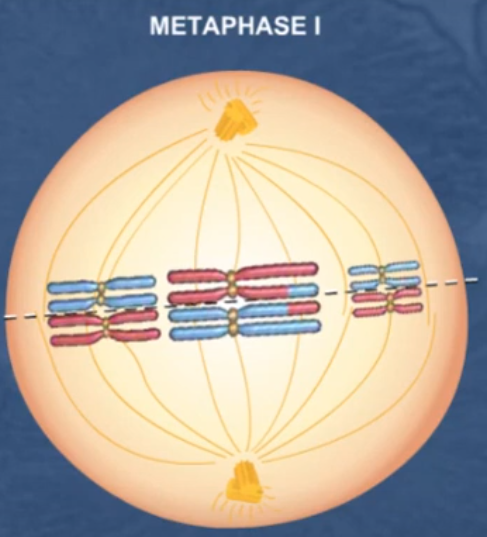
\includegraphics[width=0.4\textwidth]{metaphase-i}
\end{figure}

\subsubsection{Anaphase I (mostly same as mitosis)}
\begin{itemize}
    \item{Instead of splitting chromosomes, the homologous pairs are \textbf{segregated} (separated) and travel to opposite poles}
    \item{Diploid mother cell is now 2 haploid daughter cells}
\end{itemize}

\begin{figure}[H]
    \centering
    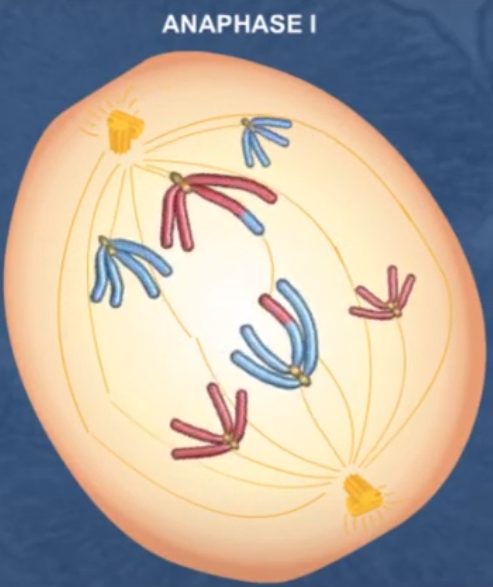
\includegraphics[width=0.4\textwidth]{anaphase-i}
\end{figure}

\subsubsection{Telophase I (same as mitosis)}
\begin{itemize}
    \item{
            The 2 cells are...
            \begin{itemize}
                \item{not identical to each other}
                \item{not identical to parent cell}
            \end{itemize}
        }
    \item{Each chromosome remains double stranded}
\end{itemize}

\subsection{Meiosis II}\noindent

Occurs at the same time in both of the daughter cells from Meiosis I.

No S phase.

\subsubsection{Same as Mitosis}
The following stages occur identically to mitosis.

\begin{itemize}
    \item{Prophase II}
    \item{Metaphase II}
    \item{Anaphase II}
    \item{Telophase II}
\end{itemize}

\subsection{Conclusion}
1 diploid mother somatic cell $\xrightarrow{\textrm{meiosis}}$ 4 haploid daughter gametes (sperm or egg)

\begin{figure}[H]
    \centering
    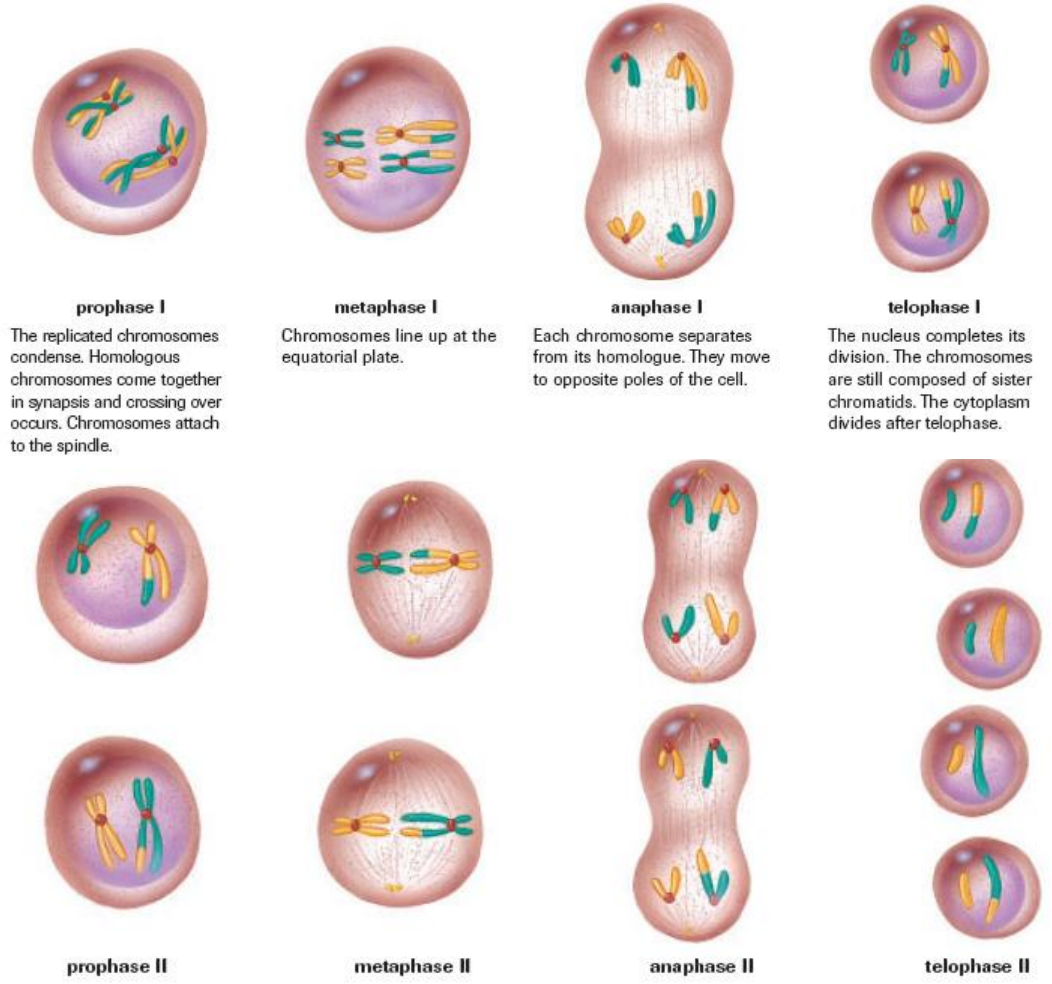
\includegraphics[width=0.9\textwidth]{meiosis}
\end{figure}

\section{Mitosis vs. Meiosis}
\begin{itemize}
    \item{\hl{Mitosis maintains} ploidy level (\# of chromosomes)}
    \item{\hl{Meiosis reduces} ploidy level}
        \\
    \item{Meiosis only occurs in gonad cells}
    \item{Mitosis is far more common}
\end{itemize}

\begin{figure}[H]
    \centering
    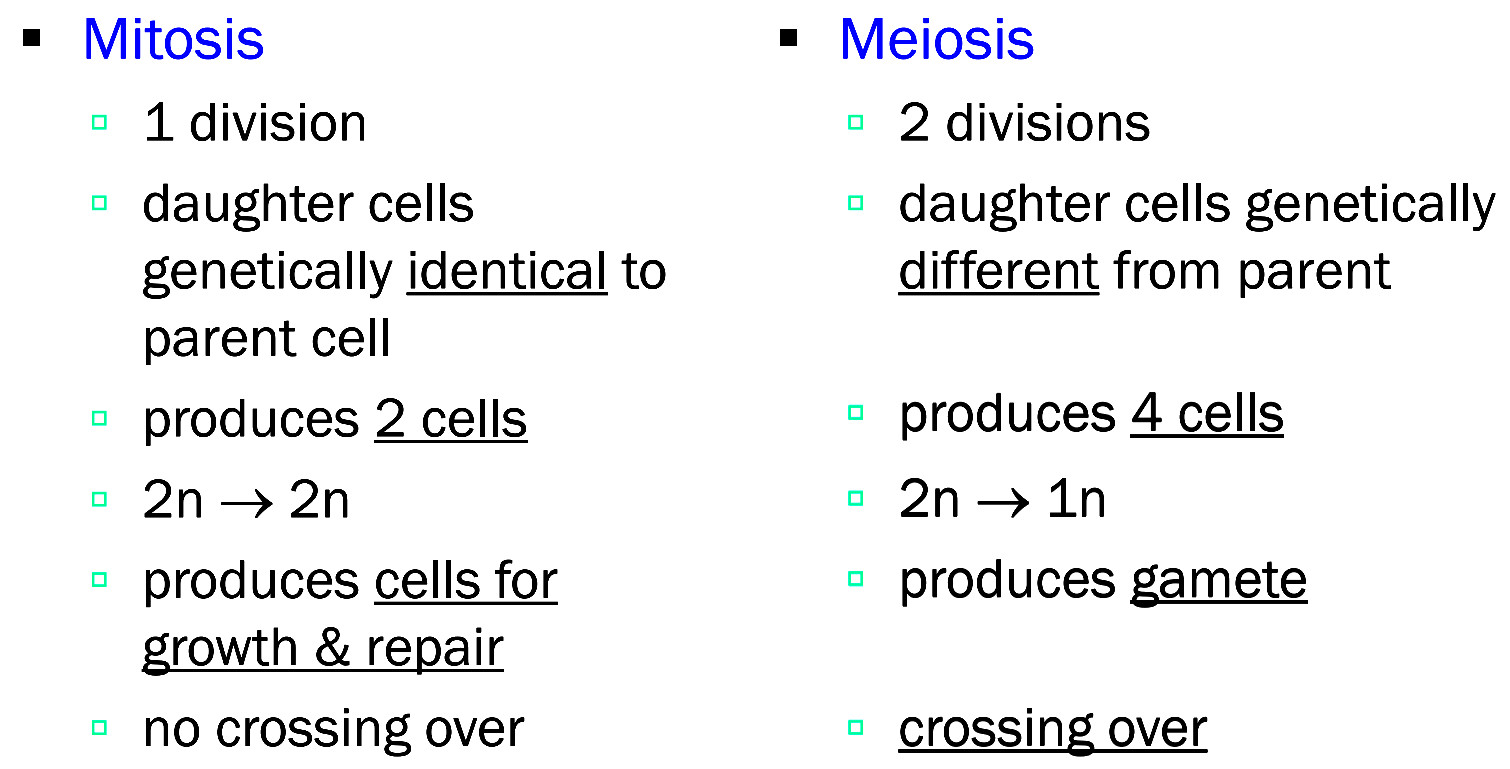
\includegraphics[width=\textwidth]{compare}
\end{figure}

\pagebreak

\section{Differences Across Kingdoms}
\subsection{Reading a Life Cycle}
You may be given the life cycle of a random species and need to identify whether a \hl{step is haploid or diplod}. Just remember the following...
\begin{itemize}
    \item{
            Mitosis
            \begin{itemize}
                \item{$2n \longrightarrow 2n$}
            \end{itemize}
        }
    \item{
            Meiosis
            \begin{itemize}
                \item{$2n \longrightarrow n$}
            \end{itemize}
        }
    \item{
            Fertilization
            \begin{itemize}
                \item{$n \longrightarrow 2n$}
            \end{itemize}
        }
\end{itemize}

\subsection{Plant Sexual Reproduction}
\begin{itemize}
    \item{
            \textbf{Alternation of Generations}
            \begin{itemize}
                \item{\textbf{Sporophyte} = non-sexual components of plant (e.g. pine tree, stem)}
                \item{\textbf{Gametophyte} = sexual components of plant (e.g. pine cone, flower)}
                \item{plant sporophyte ($2n$) and gametophyte ($n$) take turns \hl{reproducing each other}}
            \end{itemize}
        }
    \item{Pollen are \male\! male sex cells}
    \item{\female\! Eggs are stored in a variety of locations}
    \item{Fertilization results in a seed}
    \item{\hl{Sporophyte (diploid, $2n$) $\longrightarrow$ Spores (haploid, $n$) $\longrightarrow$ Gametophyte (haploid, $n$)}}
\end{itemize}

\section{Development of \male\! Male and \female\! Female Gametes}
\begin{itemize}
    \item{\textbf{Primary} = before meiosis I}
    \item{
            \textbf{Secondary} = after meiosis I
            \begin{itemize}
                \item{eggs pause during meiosis II --- specifically metaphase II --- to wait for sperm, needed to complete meiosis II}
            \end{itemize}
        }
    \item{\textbf{Gametogenesis} = formation of gametes during meiosis}
    \item{\textbf{Spermatogenesis} = formation of sperm cells}
    \item{
            \textbf{Spermatocyte} = a diploid cell that undergoes meiosis to become 4 sperm cells
            \begin{itemize}
                \item{Capable of many mitotic divisons before meiosis}
                \item{Explains males being able to produce 1 billion sperm per day}
            \end{itemize}
        }
\end{itemize}

\begin{figure}[H]
    \centering
    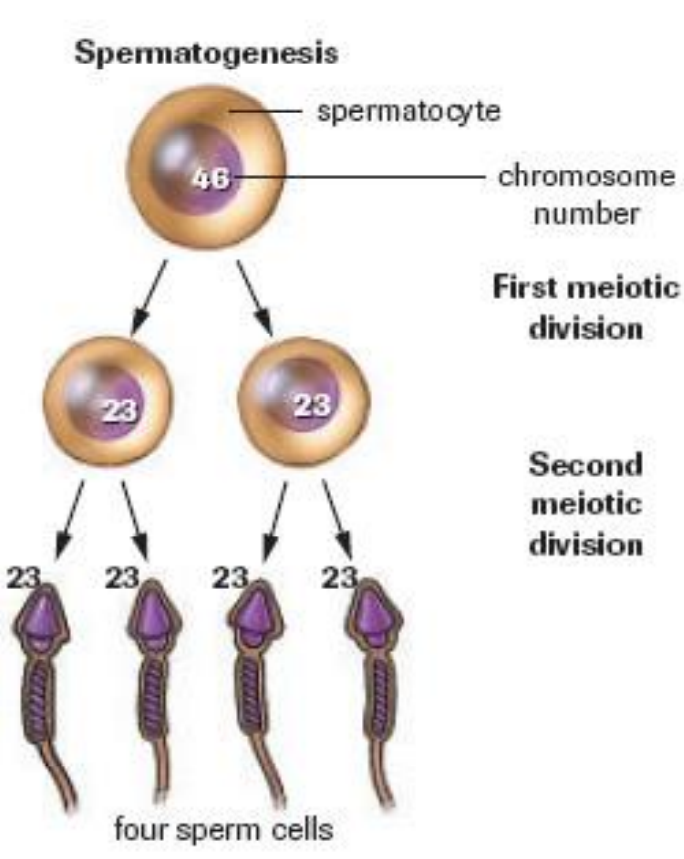
\includegraphics[width=0.5\textwidth]{spermatogenesis}
\end{figure}

\subsection{Oogenesis}
\begin{itemize}
    \item{Cytoplasm of female gametes (eggs) is \hl{not divided equally} after every division}
    \item{\textbf{Ootid} (aka. oocyte) = The one daughter cell that recieves the most cytoplasm}
    \item{\textbf{Polar Body} = The other daughter cells die, their nutrients absorbed}
    \item{Only \hl{one egg is viable} for fertilization every division}
\end{itemize}

\begin{figure}[H]
    \centering
    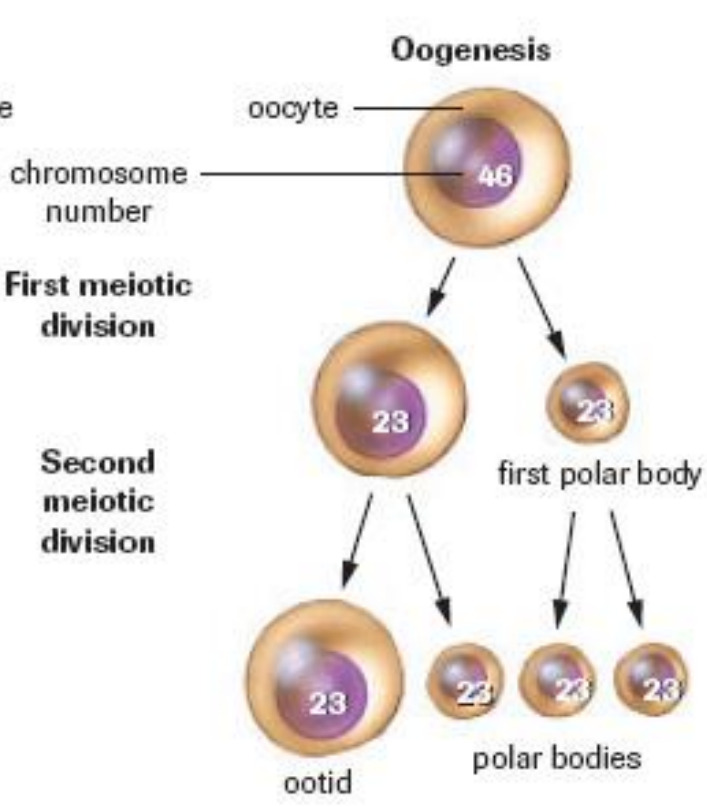
\includegraphics[width=0.4\textwidth]{oogenesis}
\end{figure}

\section{Immature $\longrightarrow$ Mature}
\begin{figure}[H]
    \centering
    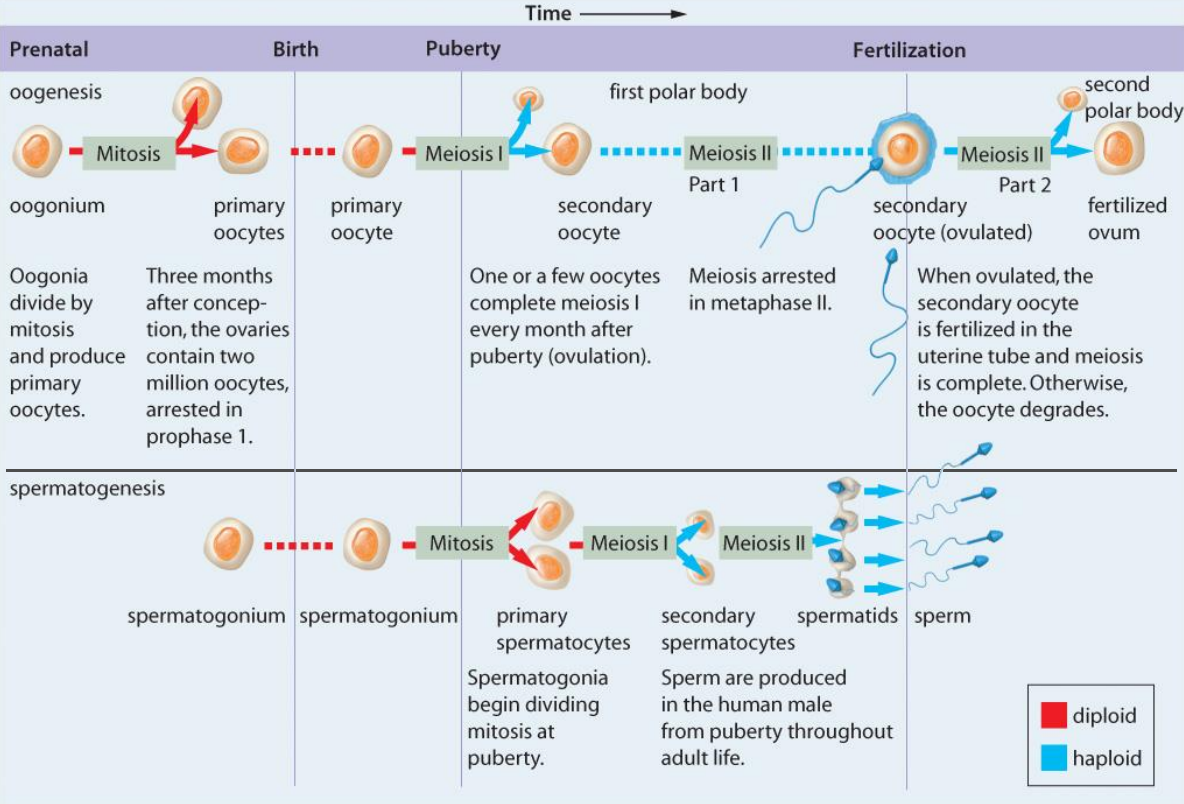
\includegraphics[width=\textwidth]{genesis}
\end{figure}

\section{(17.4) Nondisjunctions}
Also known as \textbf{abnormal meiosis}.
\begin{itemize}
    \item{Occurs when 2 homologous chromosomes \hl{move to the same pole}}
    \item{Occurs during \hl{anaphase} in mitosis, meiosis I, or meiosis II (test question)}
    \item{A cell will be missing a chromosome, and another will have an extra}
    \item{Cells with \hl{too much or too little} genetic information will \hl{not function correctly}}
\end{itemize}

\subsection{Anaphase I \& II}
Nondisjunction can occur in either anaphase I or anaphase II. The difference is...
\begin{itemize}
    \item{\textbf{Nondisjunction in anaphase \hl{I}} \\ \hl{2} cells have too many chromosomes, \hl{2} cells have too little chromosomes}
    \item{\textbf{Nondisjunction in anaphase \hl{II}} \\ \hl{1} cell has too many chromosomes, \hl{1} cell has too little chromosomes}
\end{itemize}
This is a test question.

\begin{figure}[H]
    \centering
    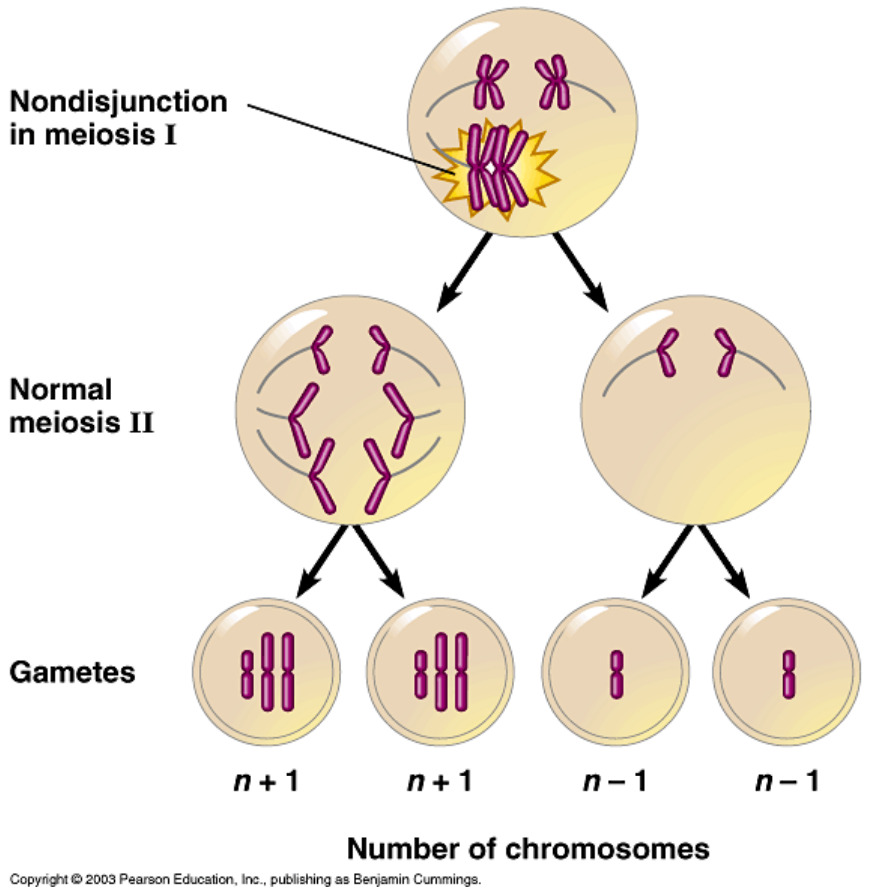
\includegraphics[width=0.45\textwidth]{nonj1}
\end{figure}

\begin{figure}[H]
    \centering
    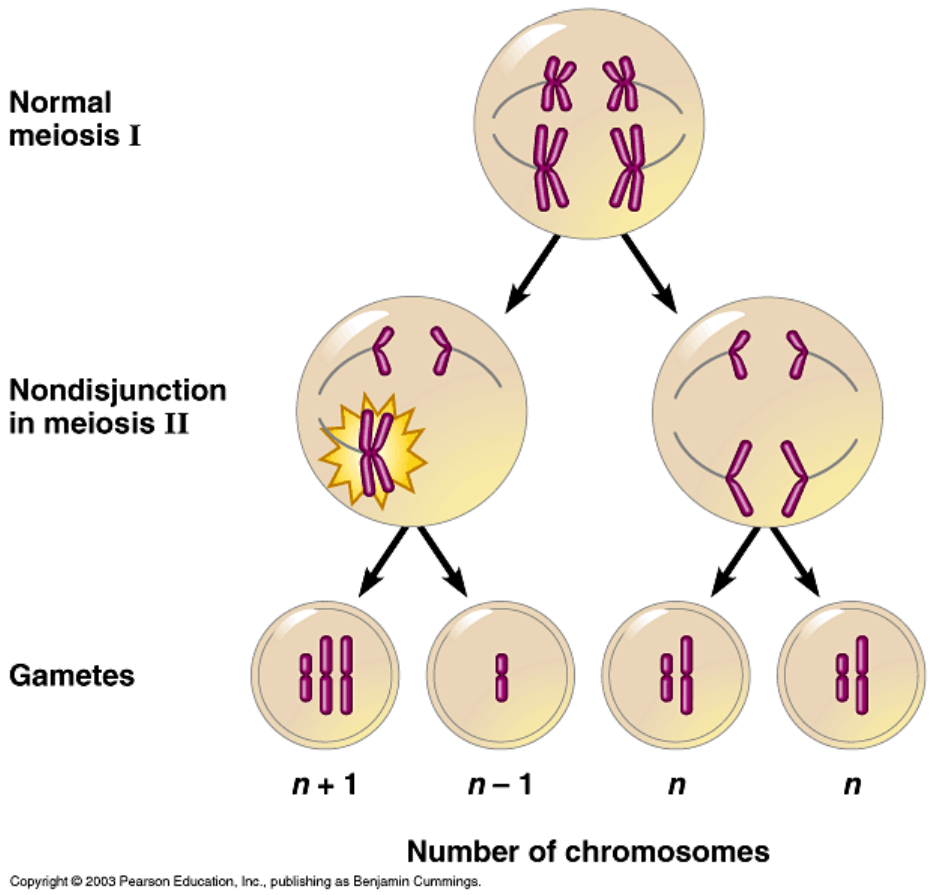
\includegraphics[width=0.45\textwidth]{nonj2}
\end{figure}

\subsection{Terms}
\begin{itemize}
    \item{\textbf{Karyotype chart} = A \hl{picture of chromosomes}, arranged in homologous pairs}
    \item{
            \textbf{Polyploidy} = An organism with \hl{$>2$ complete sets of chromosomes}
            \begin{itemize}
                \item{\textbf{Triploidy} ($3n$) = may result from abnormally diploid ($2n$) egg fertilized by normal ($n$) sperm, or vice versa}
                \item{\textbf{Tetraploidy} ($4n$) = doesn't occur in humans, failure of diploid zygote to divide after duplicating chromosomes following mitosis}
                \item{\textbf{Aneuploidy} = \hl{all cells} of the body contain \hl{abnormal \# of chromosomes}}
            \end{itemize}
        }
    \item{\textbf{Trisomy} = fertilized egg with \hl{3} \# of a chromosome (\hl{normally 2}) \\ normal gamete (23 pairs) + abnormal gamete (24 pairs), 47 chromosomes total}
    \item{\textbf{Monosomy} = fertilized egg with \hl{1} \# of a chromosome (\hl{normally 2}) \\ normal gamete (23 pairs) + abnormal gamete (22 pairs), 45 chromosomes total}
\end{itemize}

\subsection{Syndromes}

\subsubsection{Down Syndrome}
aka. \hl{Trisomy 21}

\begin{itemize}
    \item{\hl{Extra chromosome in pair \#21} (trisomic disorder)}
    \item{
            Causes...
            \begin{itemize}
                \item{mentally challenged}
                \item{round, full face}
                \item{enlarged, creased tongue}
                \item{short}
                \item{large forehead}
            \end{itemize}
        }
\end{itemize}

\begin{figure}[H]
    \centering
    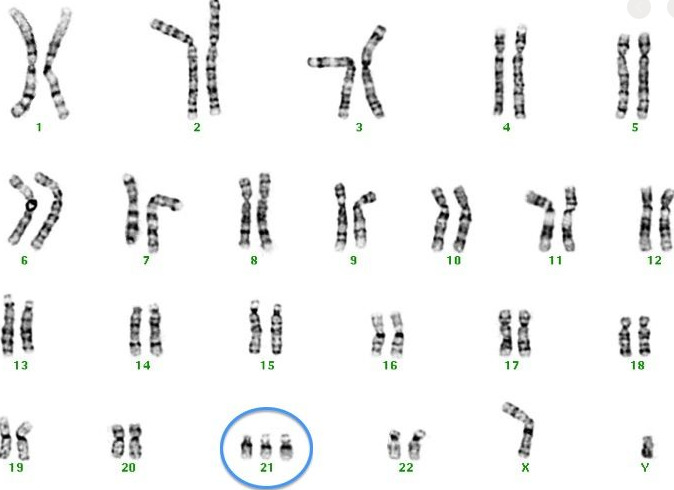
\includegraphics[width=0.75\textwidth]{down}
\end{figure}

\pagebreak

\subsubsection{Turner's Syndrome}
\begin{itemize}
    \item{\hl{Female with a single \female X chromosome (instead of \female XX)} (monosomic disorder)}
    \item{
            Causes...
            \begin{itemize}
                \item{no sexual development}
                \item{short}
                \item{thick, widened necks}
            \end{itemize}
        }
\end{itemize}

\begin{figure}[H]
    \centering
    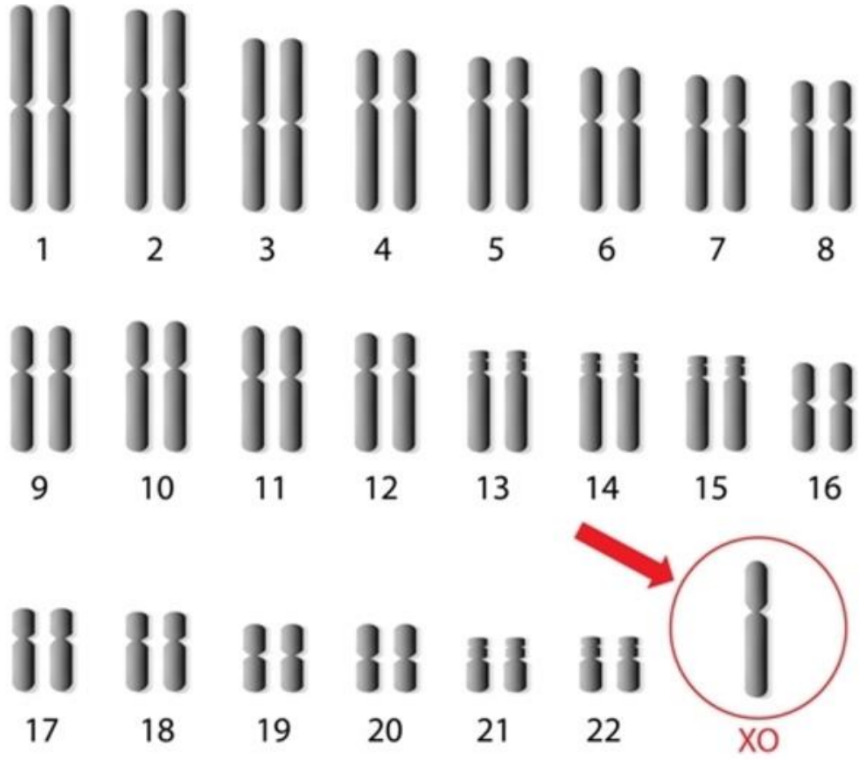
\includegraphics[width=0.55\textwidth]{turners}
\end{figure}

\subsubsection{Klinefelter Syndrome}
\begin{itemize}
    \item{\hl{Male with an extra \female X chromosome (XXY instead of XY)} (trisomic disorder)}
    \item{
            Causes...
            \begin{itemize}
                \item{high estrogen}
                \item{sterility}
            \end{itemize}
        }
\end{itemize}

\begin{figure}[H]
    \centering
    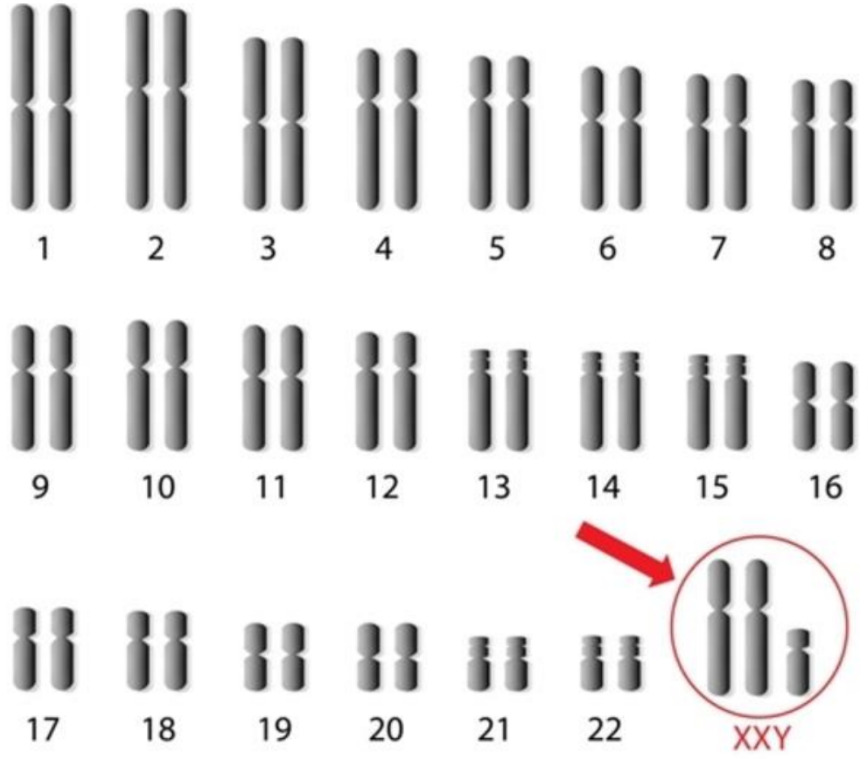
\includegraphics[width=0.55\textwidth]{klinefelter}
\end{figure}

\subsection{Teratogenic Compounds}
\begin{itemize}
    \item{Chemicals that cause abnormalities in embryos}
    \item{drugs (e.g. alcohol), infectious agents (viruses), radiation}
\end{itemize}

\section{Diagnosis of Fetus}

\subsection{Amniocentesis}
\begin{itemize}
    \item{Use of a syringe to \hl{draw fluid from sac} surrounding fetus}
    \item{Analysis can \hl{identify disorders}, \hl{down syndrome}, and \hl{sex}}
    \item{Amniotic fluid contains not a lot of cells from the fetus, so results take a while}
    \item{\textbf{Ultrasound} = used to locate position of fetus in womb}
\end{itemize}

\begin{figure}[H]
    \centering
    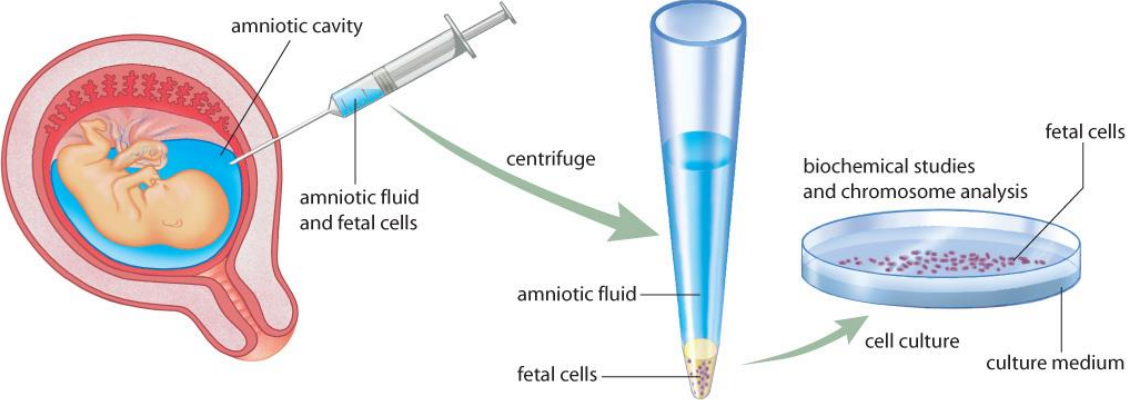
\includegraphics[width=\textwidth]{amnio}
\end{figure}

\subsection{Chorionic Villus Sampling (CVS)}
\begin{itemize}
    \item{Drawing cells from outer membrane surrounding embryo}
    \item{Can be \hl{done earlier and results quicker} than amniocentesis}
\end{itemize}

\pagebreak

\section{(20.1) DNA}
\begin{itemize}
    \item{\hl{Deoxyribonucleic Acid}}
    \item{Carrier of \hl{genetic info} and instructions that ensure \hl{continuity of life} \\ (common diploma term)}
    \item{Regulates production of cell \hl{protein}}
    \item{Only molecule that can \hl{duplicate itself}}
\end{itemize}

\subsection{Names}
\begin{itemize}
    \item{\textbf{Franklin} = female who discovered it, or something}
    \item{\textbf{Watson} \& \textbf{Crick} = guys who yoinked it and won the nobel prize}
\end{itemize}

\subsection{Basic Units}
\begin{itemize}
    \item{\textbf{Nucleotide} = basic unit of DNA}
    \item{
            Comprised of...
            \begin{itemize}
                \item{phosphates}
                \item{deoxyribose sugars}
                \item{nitrogen-containing bases}
            \end{itemize}
        }
\end{itemize}

\subsubsection{Nitrogen-Containing Bases}
\begin{itemize}
    \item{\hl{A} = \textbf{Adenine}}
    \item{\hl{T} = \textbf{Thymine}}
    \item{\hl{G} = \textbf{Guanine}}
    \item{\hl{C} = \textbf{Cytosine}}
        \\
    \item{
            The following \hl{always pair} with one another in DNA, so they are in \hl{equal quantities}
            \begin{itemize}
                \item{\# of A = \# of T}
                \item{\# of G = \# of C}
            \end{itemize}
        }
\end{itemize}

\section{Structure}
\begin{itemize}
    \item{Double helix (twisted ladder)}
    \item{Sugar and phosphate molecules form "\hl{backbone/spine}" of ladder}
    \item{N bases form \hl{rungs} of ladder}
    \item{N bases of different spines are bonded together via \hl{weak hydrogen bonds}}
\end{itemize}

\subsection{Complementary Pairs}
\begin{itemize}
    \item{N bases are always paired \hl{purine + pyrimidine}}
    \item{\textbf{Purine} = 2 ring structure (A, G)}
    \item{\textbf{Pyrimidine} = 1 ring structure (C, T, U)}
\end{itemize}

\begin{figure}[H]
    \centering
    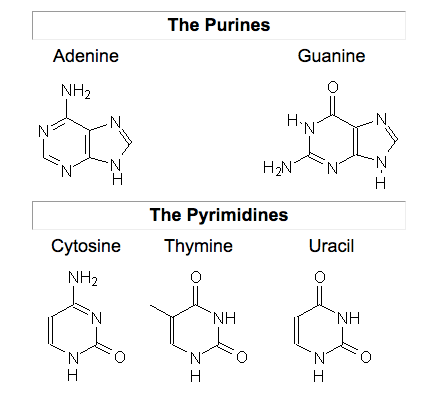
\includegraphics[width=0.40\textwidth]{ring}
\end{figure}

\subsection{Anti-Parallel}
\begin{itemize}
    \item{The strands of the double helix are parallel}
    \item{However, they run in \hl{opposite directions}, upside-down to one another}
    \item{Strands have \hl{positive and negative ends}, upside-down to balance}
\end{itemize}

\section{DNA Replication}
\begin{itemize}
    \item{DNA is duplicated during S phase interphase}
    \item{Process is semiconservative --- one strand is duplicated, the other is the old one}
\end{itemize}

\subsection{Steps (simplified)}
\begin{enumerate}
    \item{Hydrogen bonds break. DNA helix \hl{unzips}}
    \item{Each strand acts as a template to build the \hl{complementary} strand}
    \item{Errors are repaired}
    \item{Two identical copies of DNA in the end}
\end{enumerate}

\begin{figure}[H]
    \centering
    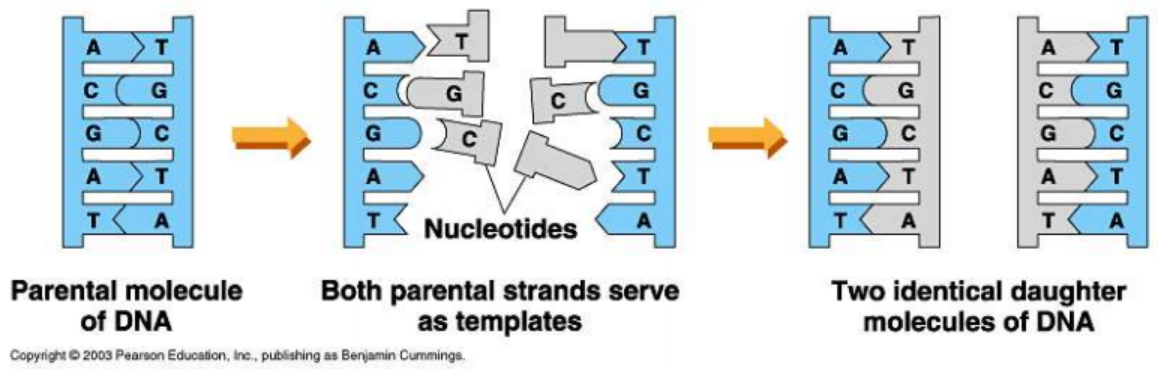
\includegraphics[width=0.7\textwidth]{replication}
\end{figure}

\subsection{Steps}
\begin{enumerate}
    \item{
            \textbf{DNA helicase} enzyme
            \begin{itemize}
                \item{\hl{Unwinds helix} by breaking \hl{hydrogen bonds} between complementary base pairs}
                \item{The point where the \hl{two strands separate} is called the \textbf{replication fork}}
            \end{itemize}
        }
    \item{
            \textbf{DNA polymerase III} enzyme
            \begin{itemize}
                \item{Links together free nucleotides (DNA from the \hl{food you eat}) that have bases \hl{complementary to the template} strand}
            \end{itemize}
        }
    \item{
            \textbf{DNA ligase} enzyme
            \begin{itemize}
                \item{The two strands of DNA from the split are treated differently}
                \item{\textbf{Leading} vs \textbf{lagging} strand}
                \item{Leading strand written continuously by DNA polymerase III, ligase not needed}
                \item{Lagging strand written in chunks}
                \item{Ligase glues together the sugar-phosphate backbone and DNA fragments/chunks in \hl{lagging strands}, \hl{filling in the gaps}}
            \end{itemize}
        }
    \item{
            \textbf{DNA polymerase I \& III} enzyme
            \begin{itemize}
                \item{Uncomplimentary N bases may become paired}
                \item{These enzymes \hl{proofread} the DNA and \hl{fix any errors/mutations} from hazardous chemicals or radiation}
            \end{itemize}
        }
\end{enumerate}

\begin{figure}[H]
    \centering
    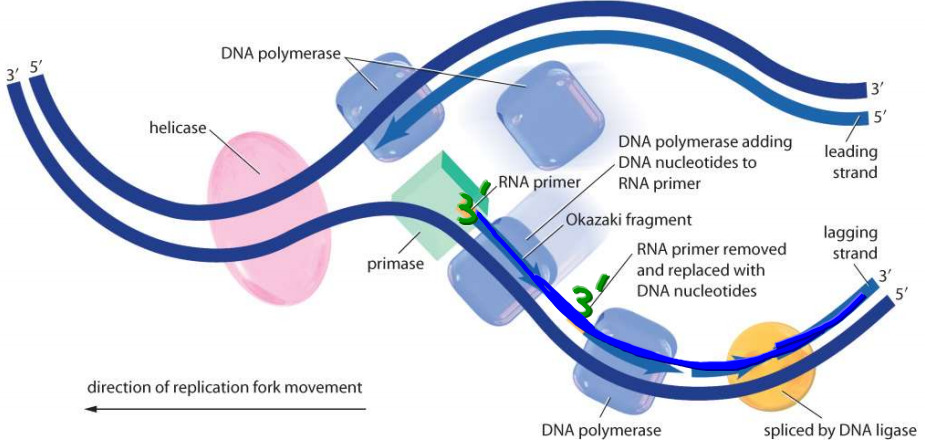
\includegraphics[width=\textwidth]{split}
\end{figure}

\pagebreak

\section{(20.2) Protein Synthesis}
\begin{itemize}
    \item{Sequence of N bases of DNA determines \hl{which proteins are made} \& the activities of proteins}
    \item{DNA \hl{too large to leave nucleus} during protein synthesis}
    \item{
            \textbf{Messenger RNA}, \textbf{mRNA}, is used instead
            \begin{itemize}
                \item{\hl{Reads} DNA code and \hl{carries} it to ribosomes}
            \end{itemize}
        }
\end{itemize}

\subsection{RNA vs. DNA}
\begin{itemize}
    \item{RNA has a \hl{ribose sugar}, instead of a deoxyribose sugar}
    \item{RNA has \hl{no thymine}; \textbf{uracil} (U) in its place}
    \item{RNA is \hl{single-stranded}, DNA is double-stranded}
\end{itemize}

\begin{figure}[H]
    \centering
    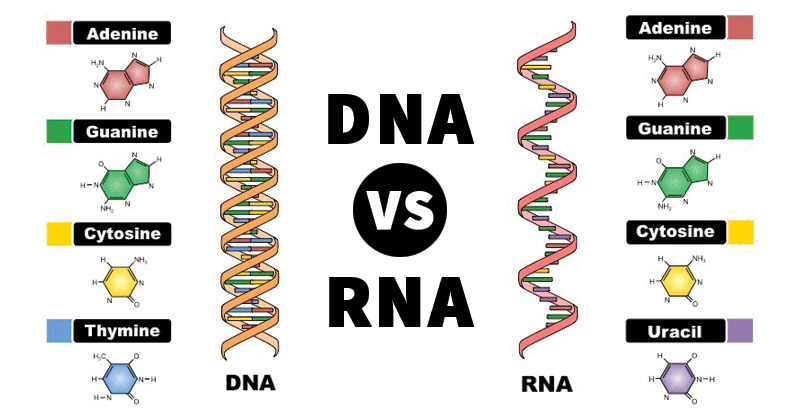
\includegraphics[width=\textwidth]{dnarna}
\end{figure}

\subsection{Steps}

\subsubsection{Transcription}
Occurs in nucleus.

\textbf{Initiation}
\begin{itemize}
    \item{RNA polymerase binds to promoter sequence (not transcribed) on DNA}
    \item{RNA polymerase allows for nucleotides to attach along mRNA}
        \\
\end{itemize}

\textbf{Elongation}
\begin{itemize}
    \item{DNA unzips}
    \item{mRNA reads single strand from the DNA, known as the \textbf{template strnad}}
    \item{
            mRNA finds complementary pair for each nucleotide on template strand
            \begin{itemize}
                \item{DNA cytosine $\longleftrightarrow$ mRNA guanine}
                \item{DNA thymine $\longrightarrow$ mRNA adenine}
                \item{DNA adenine $\longrightarrow$ mRNA uracil (RNA has no thymine, \hl{uracil instead})}
            \end{itemize}
        }
    \item{mRNA joins complementary nucleotides to a long chain}
        \\
\end{itemize}

\begin{figure}[H]
    \centering
    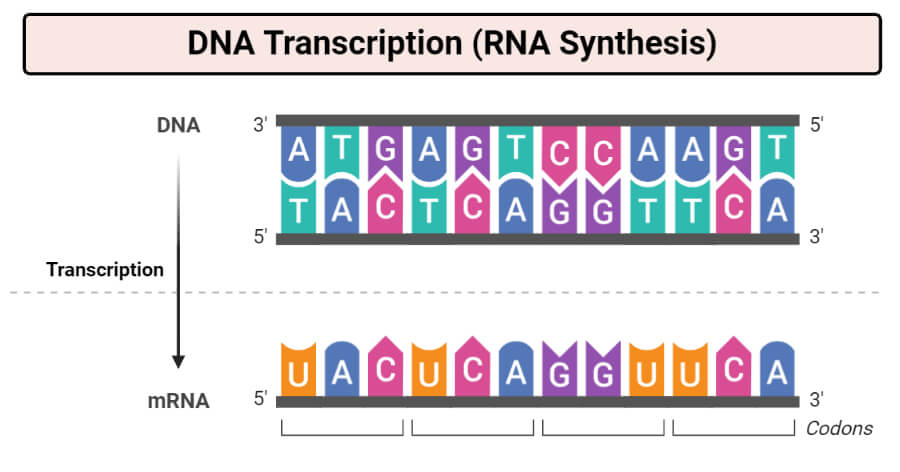
\includegraphics[width=0.7\textwidth]{transcription2}
\end{figure}

\textbf{Termination}
\begin{itemize}
    \item{mRNA moves away from DNA, disconnecting the chain it made}
    \item{2 strands of original DNA rejoin}
    \item{Single-stranded mRNA molecule moves through nuclear membrane, carrying N base code to ribosomes in cytoplasm}
\end{itemize}

\begin{figure}[H]
    \centering
    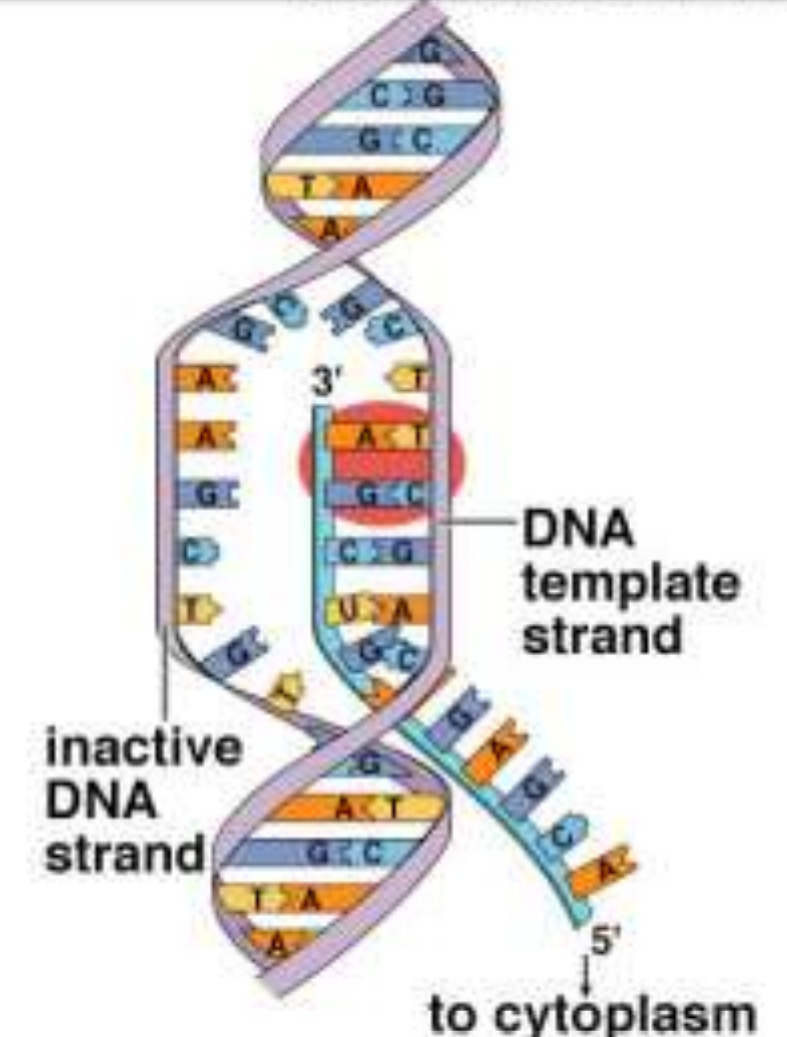
\includegraphics[width=0.50\textwidth]{transcription}
\end{figure}

\subsubsection{Translation}
Occurs in cytoplasm.

\begin{figure}[H]
    \centering
    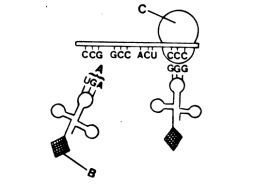
\includegraphics[width=0.50\textwidth]{translation}
    \caption{A = \textbf{Anticodon}, B = \textbf{Amino acid}, C = \textbf{Ribosome}}
\end{figure}

\textbf{Initiation}
\begin{itemize}
    \item{mRNA attaches itself to ribosomes like a ribbon}
    \item{\textbf{Codon} = \hl{3 nucleotides} that are \hl{code for an amino acid}}
    \item{\textbf{Initiator codon} turns on protein synthesis (\textbf{AUG}, \hl{methionine}, always at beginning)}
    \item{
            mRNA codons
            \begin{itemize}
                \item{Codons --- blocks of 3 nucleotides --- are decoded into a sequence of amino acids}
                \item{Nucleotide sequence to amino acid conversion table is located on \hl{page 3 on the data sheet}}
            \end{itemize}
        }
\end{itemize}

\textbf{Elongation}
\begin{itemize}
    \item{\textbf{Transfer RNA} (tRNA) picks up amino acids in cytoplasm and sends to mRNA}
    \item{mRNA codon and tRNA anticodon are \hl{complementary}}
    \item{tRNA molecule is \hl{T-shaped}}
    \item{Amino acids --- brought by tRNA --- are fused into long-chain proteins at ribosome on the top of each tRNA that brings each amino acid}
    \item{\hl{Amino acids are bonded} together by \textbf{ribosomal RNA} (rRNA)}
\end{itemize}

\textbf{Termination}
\begin{itemize}
    \item{\textbf{Terminator codon} turns synthesis off, always at the end}
    \item{
            Terminator codon can be either...
            \begin{itemize}
                \item{\textbf{UAA}}
                \item{\textbf{UGA}}
                \item{\textbf{UAG}}
            \end{itemize}
        }
\end{itemize}

\subsection{Central Dogma}
\begin{figure}[H]
    \centering
    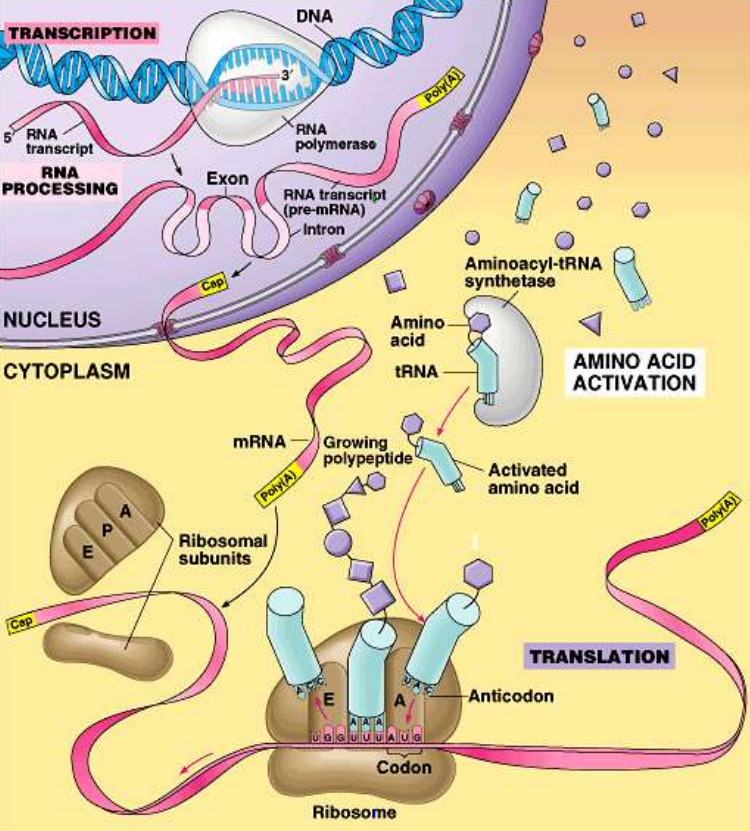
\includegraphics[width=\textwidth]{dogma}
\end{figure}

\begin{itemize}
    \item{\textbf{Central Dogma} = main idea, diploma term}
    \item{\hl{A DNA sequence encodes an RNA sequence that encodes protein}}
\end{itemize}

\subsection{Code Format Summary}
\begin{itemize}
    \item{DNA $\longleftarrow\!\!($complementary, $\textrm{T} \longleftrightarrow \textrm{U}$$)\!\!\longrightarrow$ mRNA $\longleftarrow\!\!($complementary$)\!\!\longrightarrow$ tRNA}
    \item{DNA $\longleftarrow\!\!(\textrm{T} \longleftrightarrow \textrm{U})\!\!\longrightarrow$ tRNA}
\end{itemize}

\section{(20.3) Biotechnology}

\subsection{Genetically Modified Organisms (GMO)}
\begin{itemize}
    \item{\textbf{Recombinant DNA} = piece of DNA composed of sequences from 2+ \hl{different sources}}
    \item{\textbf{Genetic transformation} = introduction and expression of foreign DNA in a living organism}
\end{itemize}

\subsubsection{Steps}
\begin{itemize}
    \item{\textbf{Restriction endonucleases/enzymes} = cut DNA at a specific base, specific \hl{recognition site}}
    \item{\textbf{Recognition site} = 4-8 base pairs long, restriction enzyme scans DNA until recognition site (e.g. Eco R1)}
    \item{Cuts on both strands, so one strand will be longer than the other; this "overhang" is called a \textbf{sticky end} (diploma term)}
\end{itemize}

\begin{figure}[H]
    \centering
    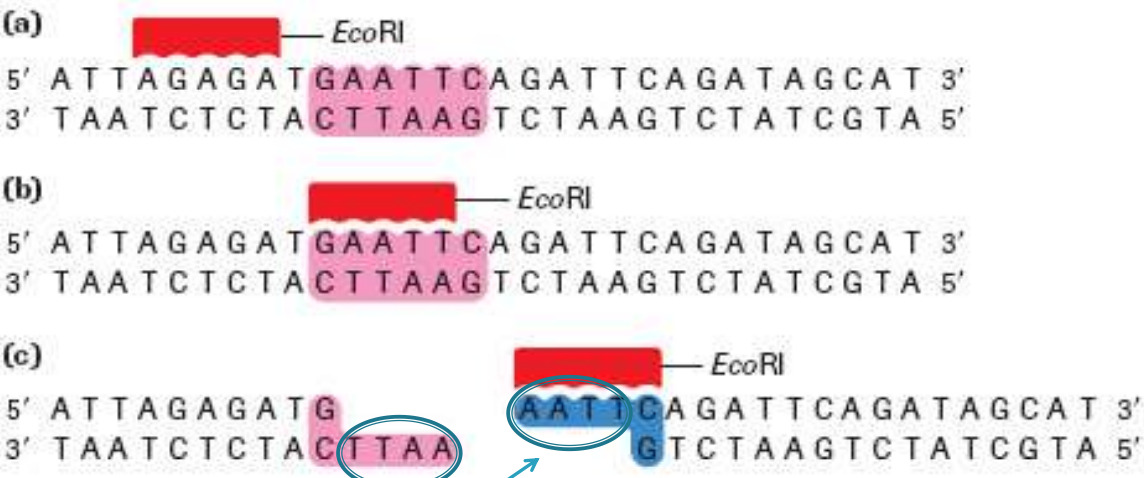
\includegraphics[width=0.75\textwidth]{rest}
    \caption{"Sticky ends" circled}
\end{figure}

\begin{itemize}
    \item{\textbf{anneal} = glue/join (diploma term)}
    \item{\textbf{DNA ligase} = foreign DNA is inserted between sticky ends and \hl{anneled} to them}
    \item{
            \textbf{Methylases}
            \begin{itemize}
                \item{Enzymes that can \hl{modify a restriction enzyme recognition site}}
                \item{Add methyl group to one of bases in site to protect its own DNA from digestion by its own restriction enzymes}
            \end{itemize}
        }
\end{itemize}

\subsection{Transgenic Bacteria}
\begin{itemize}
    \item{Annealing bacteria \hl{plasmids} in order to force them to do our bidding}
    \item{Most popular example is annealing \hl{insulin producing} DNA into bacteria plasmids}
    \item{This forces the bacteria to produce insulin, rather than harvesting it from animals}
    \item{Other examples include bacteria that eat toxic waste}
\end{itemize}

\begin{figure}[H]
    \centering
    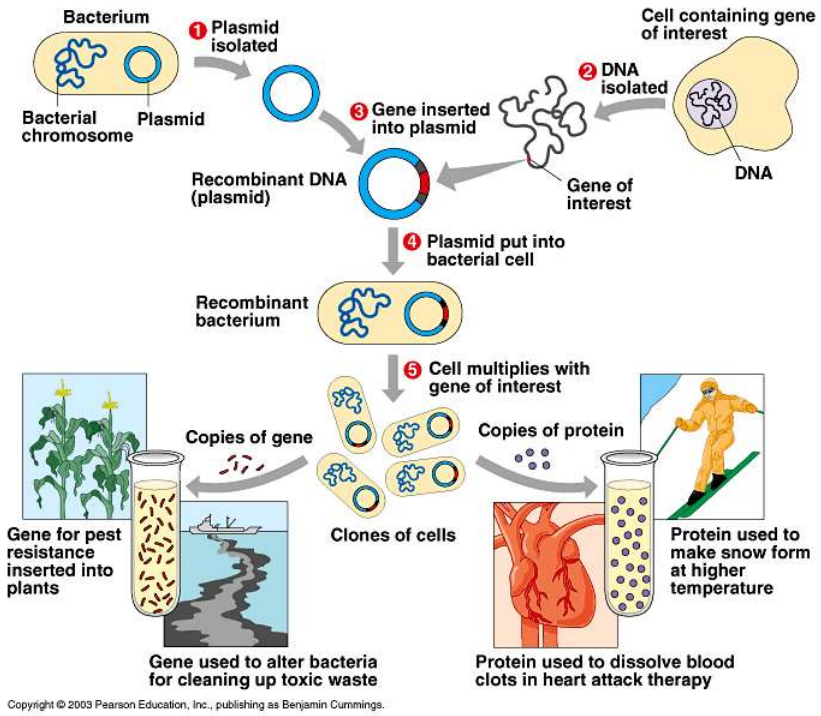
\includegraphics[width=0.75\textwidth]{plasmid}
\end{figure}

\subsection{Polymerase Chain Reaction (PCR) with Taq DNA Polymerase}
\begin{itemize}
    \item{Allows billions of \hl{copies from small quantities} of DNA}
    \item{\hl{Stable at high temperatures}}
\end{itemize}

\subsubsection{Steps (simplified)}
\begin{itemize}
    \item{DNA heated to break hydrogen bonds}
    \item{Cooled, primers form hydrogen bonds with DNA templates}
    \item{Taq polymerase creates new DNA strand using template via complementary base pairing, starting at each primer}
    \item{Repeat for more DNA copies}
\end{itemize}

\begin{figure}[H]
    \centering
    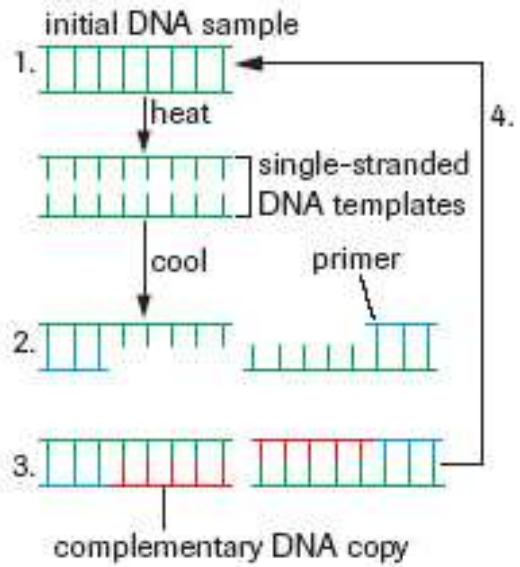
\includegraphics[width=0.25\textwidth]{taq}
\end{figure}

\subsection{DNA Fingerprint Test}
At the Alberta level, all you would be tested on is...
\begin{itemize}
    \item{Matching the black bands --- called \textbf{RFLP}s --- of the DNA samples}
    \item{Identify which sample is more similar}
\end{itemize}


\section{(20.4) Mutations}
\begin{itemize}
    \item{Changes in a sequence of DNA}
    \item{
            \textbf{Mutagenic agents} = things that \hl{alter DNA}
            \begin{itemize}
                \item{cosmic rays}
                \item{x-rays}
                \item{UV radiation}
                \item{chemicals}
            \end{itemize}
            Especially harmful during \hl{1st trimester of pregnancy}
        }
    \item{Gamete mutations lead to permanent change in offspring characteristics}
\end{itemize}

\subsection{Classes}
\begin{itemize}
    \item{\textbf{Beneficial mutations} = selective advantage, tends to become more common over time, leads to evolutionary change}
    \item{\textbf{Harmful mutations} = reduces an individual's fitness, tends to be selected against, occurs at low rates}
    \item{\textbf{Neutral mutations} = no benefit nor cost, not acted on by natural selection}
\end{itemize}

\subsection{Point Mutations}
Changes a \hl{single base pair} in DNA.

\begin{figure}[H]
    \centering
    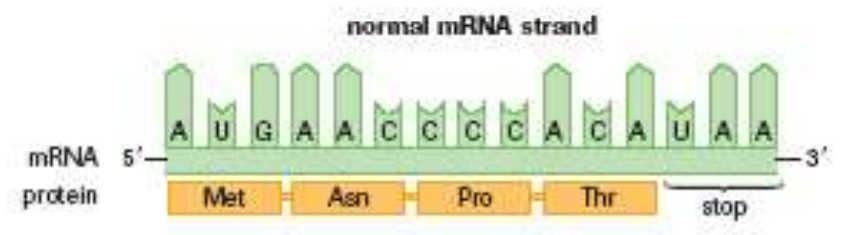
\includegraphics[width=0.50\textwidth]{original}
\end{figure}

\begin{itemize}
    \item{
            \textbf{Silent mutatation} = no effect; \hl{doesn't change amino acid} coded for
            \begin{figure}[H]
                \centering
                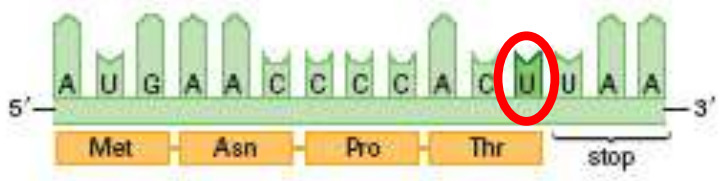
\includegraphics[width=0.50\textwidth]{silent}
            \end{figure}
        }
    \item{
            \textbf{Missense mutatation} = \hl{changes one amino acid} coded for; e.g. sickle-cell anemia
            \begin{figure}[H]
                \centering
                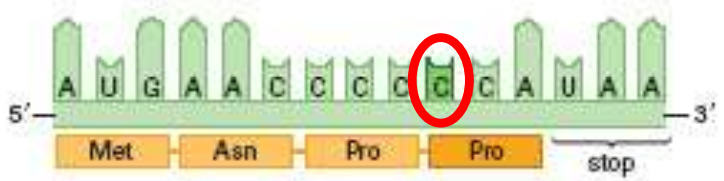
\includegraphics[width=0.50\textwidth]{missense}
            \end{figure}
        }
    \item{
            \textbf{Nonsense mutatation} = converts an amino acid codon \hl{into a stop codon}, part of protein may be digested by cell proteases, often lethal
            \begin{figure}[H]
                \centering
                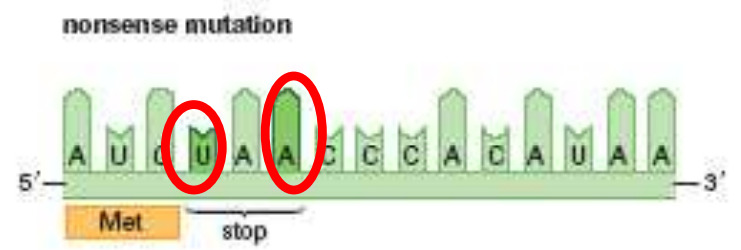
\includegraphics[width=0.50\textwidth]{nonsense}
            \end{figure}
        }
\end{itemize}

\subsection{Gene Mutations}
\begin{itemize}
    \item{Changes the amino acids specified by DNA sequence}
    \item{May involve \hl{1 or more base pairs}}
    \item{Both cause \textbf{frameshift mutations}, shifting all the nucleotides, causing completely different codons to be read}
\end{itemize}

\begin{itemize}
    \item{
            \textbf{Deletion mutation} = 1 or more nucleotides removed from DNA sequence
            \begin{figure}[H]
                \centering
                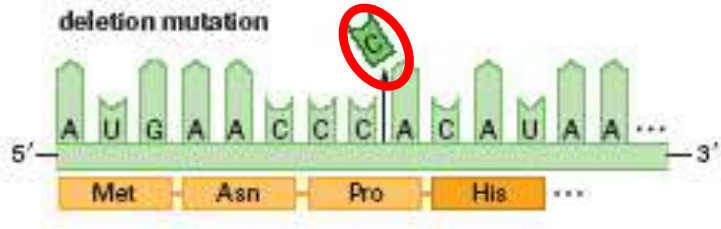
\includegraphics[width=0.50\textwidth]{deletion}
            \end{figure}

            \begin{figure}[H]
                \centering
                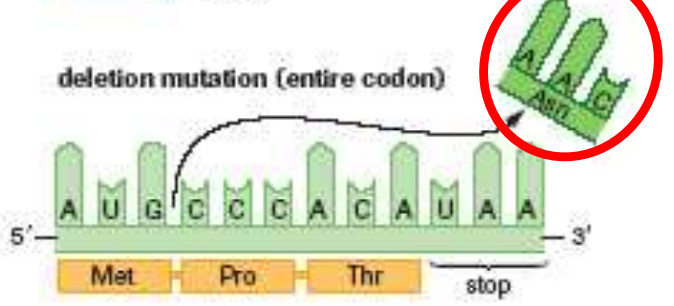
\includegraphics[width=0.50\textwidth]{deletion2}
            \end{figure}
        }
    \item{
            \textbf{Insertion mutation} = extra nucleotide inserted into DNA
            \begin{figure}[H]
                \centering
                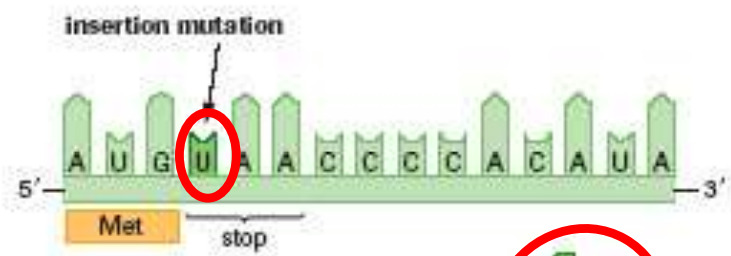
\includegraphics[width=0.50\textwidth]{insertion}
            \end{figure}
        }
\end{itemize}

\subsection{Chromosomal Mutations}
Involves large segments of DNA

\begin{itemize}
    \item{
            \textbf{Translocation} = relocation of groups of base pairs from 1 part of a genome to another
            \begin{figure}[H]
                \centering
                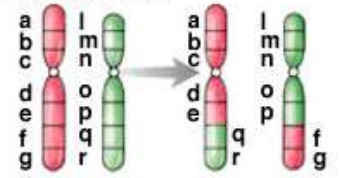
\includegraphics[width=0.3\textwidth]{translocation}
            \end{figure}
        }
    \item{
            \textbf{Inversion} = section of chromosome reversed in orientation
            \begin{figure}[H]
                \centering
                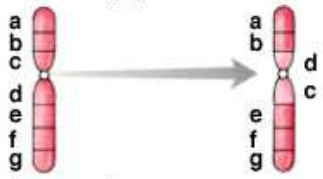
\includegraphics[width=0.3\textwidth]{inversion}
            \end{figure}
        }
\end{itemize}
\begin{figure}[H]
    \centering
    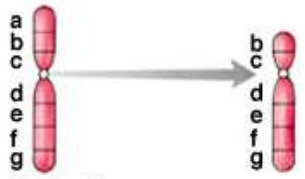
\includegraphics[width=0.3\textwidth]{deletion3}
    \caption{Deletion}
\end{figure}
\begin{figure}[H]
    \centering
    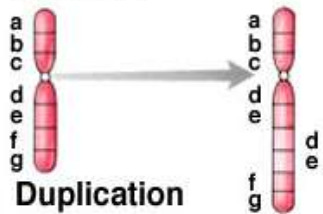
\includegraphics[width=0.3\textwidth]{duplication}
    \caption{Duplication}
\end{figure}

\subsection{Mutation Examples}
\begin{itemize}
    \item{\textbf{Hemophilia} = absence of protein needed for blood clotting}
    \item{\textbf{Cystic fibrosis} = deletion; inability to produce protein that regulates $Cl^-$ channels, lung secretions \hl{thick and block airways}}
\end{itemize}

\subsection{Causes}
\begin{itemize}
    \item{\textbf{Spontaneous mutations} = errors made in DNA replication, DNA polymerase I, results in point mutation}
    \item{Mutagenic agents}
\end{itemize}

\section{Oncogenes}
\begin{itemize}
    \item{'onco-' = cancer}
    \item{Cancer-causing genes}
    \item{\hl{Present in normal} strands of DNA}
    \item{\hl{Regulator gene} keeps oncogenes turned off}
    \item{Translocation allows oncogene to \hl{turn itself on}}
\end{itemize}

\section{Mitochondrial DNA (mtDNA)}
\begin{itemize}
    \item{identical to one's mother's mtDNA}
    \item{\textbf{Eve Project} = tracing mutations in mtDNA, shows ancestry}
\end{itemize}

\pagebreak

\section{IB TOPICS}
In your booklet. :)

\end{document}
